\documentclass{article}



\usepackage{arxiv}

\usepackage[utf8]{inputenc} % allow utf-8 input
\usepackage[T1]{fontenc}    % use 8-bit T1 fonts
\usepackage{hyperref}       % hyperlinks
\usepackage{url}            % simple URL typesetting
\usepackage{booktabs}       % professional-quality tables
\usepackage{amsfonts}       % blackboard math symbols
\usepackage{nicefrac}       % compact symbols for 1/2, etc.
\usepackage{microtype}      % microtypography
\usepackage{lipsum}		% Can be removed after putting your text content
\usepackage{graphicx}
\usepackage[numbers]{natbib}
\usepackage{doi}
\usepackage{subfigure}

\usepackage{algorithm}
\usepackage{algorithmic}
\usepackage{tikz}
\usetikzlibrary{shapes.geometric, arrows, positioning}
\tikzstyle{startstop} = [rectangle, rounded corners, minimum width=3cm, minimum height=1cm, text centered, draw=black, fill=red!30]
\tikzstyle{process} = [rectangle, minimum width=3cm, minimum height=1cm, text centered, draw=black, fill=blue!30]
\tikzstyle{arrow} = [thick,->,>=stealth]
\tikzstyle{label} = [font=\small, align=center]
\usepackage{pifont}   % To use check marks and crosses


\newcommand{\cmark}{\ding{51}} % Define check mark
\newcommand{\xmark}{\ding{55}} % Define cross mark
\usepackage{amssymb}
\usepackage{mathtools}
\usepackage{amsthm}

\usepackage{pgfplots}
\usepackage{xfrac}
\usepackage{enumitem}


\usepackage{commath}
\usepackage{amsmath}
\usepackage{pgfplots}
\usepackage{xfrac}
\usepackage{amsfonts}
\usepackage{enumitem}
\usepackage{physics}
\usepackage{todonotes}
\usepackage{adjustbox}
\usepackage{multirow}
\usepackage{makecell}
\usepackage{filecontents}
\usepackage{caption}

\newcommand{\REFLOW}{\texttt{\textsc{REFLOW}}}
\usepackage[capitalize,noabbrev]{cleveref}

\usepgfplotslibrary{fillbetween}
\usepgfplotslibrary{groupplots}



% \title{On the Emergence of Signal Collapse in One-Shot Neural Network Pruning: When Sparse Models Lose Sight of Their Inputs}
%\title{On the Emergence of Signal Collapse in One-Shot Neural Network Pruning: When Sparse Models Lose Distinctions in Neural Representations}

\title{Signal Collapse in One-Shot Pruning: When Sparse Models Fail to Distinguish Neural Representations}

%\date{September 9, 1985}	% Here you can change the date presented in the paper title
%\date{} 					% Or removing it

\author{
Dhananjay Saikumar \\
School of Computer Science\\
University of St Andrews\\
St Andrews, UK, KY16 9SX\\
\texttt{ds304@st-andrews.ac.uk}
\And
Blesson Varghese \\
School of Computer Science\\
University of St Andrews\\
St Andrews, UK, KY16 9SX\\
\texttt{blesson@st-andrews.ac.uk}
}


\hypersetup{
pdftitle={A template for the arxiv style},
pdfsubject={q-bio.NC, q-bio.QM},
pdfauthor={David S.~Hippocampus, Elias D.~Striatum},
pdfkeywords={First keyword, Second keyword, More},
}

\begin{document}
\maketitle
\thispagestyle{empty}  % Removes the title from the first page header
\pagestyle{plain}      % Ensures no title in headers on subsequent pages
\begin{abstract}  
Test time scaling is currently one of the most active research areas that shows promise after training time scaling has reached its limits.
Deep-thinking (DT) models are a class of recurrent models that can perform easy-to-hard generalization by assigning more compute to harder test samples.
However, due to their inability to determine the complexity of a test sample, DT models have to use a large amount of computation for both easy and hard test samples.
Excessive test time computation is wasteful and can cause the ``overthinking'' problem where more test time computation leads to worse results.
In this paper, we introduce a test time training method for determining the optimal amount of computation needed for each sample during test time.
We also propose Conv-LiGRU, a novel recurrent architecture for efficient and robust visual reasoning. 
Extensive experiments demonstrate that Conv-LiGRU is more stable than DT, effectively mitigates the ``overthinking'' phenomenon, and achieves superior accuracy.
\end{abstract}  



% keywords can be removed
% \keywords{First keyword \and Second keyword \and More}


\section{Introduction}
\label{sec:introduction}
\section{Introduction}
\label{sec:introduction}
The business processes of organizations are experiencing ever-increasing complexity due to the large amount of data, high number of users, and high-tech devices involved \cite{martin2021pmopportunitieschallenges, beerepoot2023biggestbpmproblems}. This complexity may cause business processes to deviate from normal control flow due to unforeseen and disruptive anomalies \cite{adams2023proceddsriftdetection}. These control-flow anomalies manifest as unknown, skipped, and wrongly-ordered activities in the traces of event logs monitored from the execution of business processes \cite{ko2023adsystematicreview}. For the sake of clarity, let us consider an illustrative example of such anomalies. Figure \ref{FP_ANOMALIES} shows a so-called event log footprint, which captures the control flow relations of four activities of a hypothetical event log. In particular, this footprint captures the control-flow relations between activities \texttt{a}, \texttt{b}, \texttt{c} and \texttt{d}. These are the causal ($\rightarrow$) relation, concurrent ($\parallel$) relation, and other ($\#$) relations such as exclusivity or non-local dependency \cite{aalst2022pmhandbook}. In addition, on the right are six traces, of which five exhibit skipped, wrongly-ordered and unknown control-flow anomalies. For example, $\langle$\texttt{a b d}$\rangle$ has a skipped activity, which is \texttt{c}. Because of this skipped activity, the control-flow relation \texttt{b}$\,\#\,$\texttt{d} is violated, since \texttt{d} directly follows \texttt{b} in the anomalous trace.
\begin{figure}[!t]
\centering
\includegraphics[width=0.9\columnwidth]{images/FP_ANOMALIES.png}
\caption{An example event log footprint with six traces, of which five exhibit control-flow anomalies.}
\label{FP_ANOMALIES}
\end{figure}

\subsection{Control-flow anomaly detection}
Control-flow anomaly detection techniques aim to characterize the normal control flow from event logs and verify whether these deviations occur in new event logs \cite{ko2023adsystematicreview}. To develop control-flow anomaly detection techniques, \revision{process mining} has seen widespread adoption owing to process discovery and \revision{conformance checking}. On the one hand, process discovery is a set of algorithms that encode control-flow relations as a set of model elements and constraints according to a given modeling formalism \cite{aalst2022pmhandbook}; hereafter, we refer to the Petri net, a widespread modeling formalism. On the other hand, \revision{conformance checking} is an explainable set of algorithms that allows linking any deviations with the reference Petri net and providing the fitness measure, namely a measure of how much the Petri net fits the new event log \cite{aalst2022pmhandbook}. Many control-flow anomaly detection techniques based on \revision{conformance checking} (hereafter, \revision{conformance checking}-based techniques) use the fitness measure to determine whether an event log is anomalous \cite{bezerra2009pmad, bezerra2013adlogspais, myers2018icsadpm, pecchia2020applicationfailuresanalysispm}. 

The scientific literature also includes many \revision{conformance checking}-independent techniques for control-flow anomaly detection that combine specific types of trace encodings with machine/deep learning \cite{ko2023adsystematicreview, tavares2023pmtraceencoding}. Whereas these techniques are very effective, their explainability is challenging due to both the type of trace encoding employed and the machine/deep learning model used \cite{rawal2022trustworthyaiadvances,li2023explainablead}. Hence, in the following, we focus on the shortcomings of \revision{conformance checking}-based techniques to investigate whether it is possible to support the development of competitive control-flow anomaly detection techniques while maintaining the explainable nature of \revision{conformance checking}.
\begin{figure}[!t]
\centering
\includegraphics[width=\columnwidth]{images/HIGH_LEVEL_VIEW.png}
\caption{A high-level view of the proposed framework for combining \revision{process mining}-based feature extraction with dimensionality reduction for control-flow anomaly detection.}
\label{HIGH_LEVEL_VIEW}
\end{figure}

\subsection{Shortcomings of \revision{conformance checking}-based techniques}
Unfortunately, the detection effectiveness of \revision{conformance checking}-based techniques is affected by noisy data and low-quality Petri nets, which may be due to human errors in the modeling process or representational bias of process discovery algorithms \cite{bezerra2013adlogspais, pecchia2020applicationfailuresanalysispm, aalst2016pm}. Specifically, on the one hand, noisy data may introduce infrequent and deceptive control-flow relations that may result in inconsistent fitness measures, whereas, on the other hand, checking event logs against a low-quality Petri net could lead to an unreliable distribution of fitness measures. Nonetheless, such Petri nets can still be used as references to obtain insightful information for \revision{process mining}-based feature extraction, supporting the development of competitive and explainable \revision{conformance checking}-based techniques for control-flow anomaly detection despite the problems above. For example, a few works outline that token-based \revision{conformance checking} can be used for \revision{process mining}-based feature extraction to build tabular data and develop effective \revision{conformance checking}-based techniques for control-flow anomaly detection \cite{singh2022lapmsh, debenedictis2023dtadiiot}. However, to the best of our knowledge, the scientific literature lacks a structured proposal for \revision{process mining}-based feature extraction using the state-of-the-art \revision{conformance checking} variant, namely alignment-based \revision{conformance checking}.

\subsection{Contributions}
We propose a novel \revision{process mining}-based feature extraction approach with alignment-based \revision{conformance checking}. This variant aligns the deviating control flow with a reference Petri net; the resulting alignment can be inspected to extract additional statistics such as the number of times a given activity caused mismatches \cite{aalst2022pmhandbook}. We integrate this approach into a flexible and explainable framework for developing techniques for control-flow anomaly detection. The framework combines \revision{process mining}-based feature extraction and dimensionality reduction to handle high-dimensional feature sets, achieve detection effectiveness, and support explainability. Notably, in addition to our proposed \revision{process mining}-based feature extraction approach, the framework allows employing other approaches, enabling a fair comparison of multiple \revision{conformance checking}-based and \revision{conformance checking}-independent techniques for control-flow anomaly detection. Figure \ref{HIGH_LEVEL_VIEW} shows a high-level view of the framework. Business processes are monitored, and event logs obtained from the database of information systems. Subsequently, \revision{process mining}-based feature extraction is applied to these event logs and tabular data input to dimensionality reduction to identify control-flow anomalies. We apply several \revision{conformance checking}-based and \revision{conformance checking}-independent framework techniques to publicly available datasets, simulated data of a case study from railways, and real-world data of a case study from healthcare. We show that the framework techniques implementing our approach outperform the baseline \revision{conformance checking}-based techniques while maintaining the explainable nature of \revision{conformance checking}.

In summary, the contributions of this paper are as follows.
\begin{itemize}
    \item{
        A novel \revision{process mining}-based feature extraction approach to support the development of competitive and explainable \revision{conformance checking}-based techniques for control-flow anomaly detection.
    }
    \item{
        A flexible and explainable framework for developing techniques for control-flow anomaly detection using \revision{process mining}-based feature extraction and dimensionality reduction.
    }
    \item{
        Application to synthetic and real-world datasets of several \revision{conformance checking}-based and \revision{conformance checking}-independent framework techniques, evaluating their detection effectiveness and explainability.
    }
\end{itemize}

The rest of the paper is organized as follows.
\begin{itemize}
    \item Section \ref{sec:related_work} reviews the existing techniques for control-flow anomaly detection, categorizing them into \revision{conformance checking}-based and \revision{conformance checking}-independent techniques.
    \item Section \ref{sec:abccfe} provides the preliminaries of \revision{process mining} to establish the notation used throughout the paper, and delves into the details of the proposed \revision{process mining}-based feature extraction approach with alignment-based \revision{conformance checking}.
    \item Section \ref{sec:framework} describes the framework for developing \revision{conformance checking}-based and \revision{conformance checking}-independent techniques for control-flow anomaly detection that combine \revision{process mining}-based feature extraction and dimensionality reduction.
    \item Section \ref{sec:evaluation} presents the experiments conducted with multiple framework and baseline techniques using data from publicly available datasets and case studies.
    \item Section \ref{sec:conclusions} draws the conclusions and presents future work.
\end{itemize}


\section{Background \& Related Work}
\label{sec:relatedwork}
\section{Related Work}
The landscape of large language model vulnerabilities has been extensively studied in recent literature \cite{crothers2023machinegeneratedtextcomprehensive,shayegani2023surveyvulnerabilitieslargelanguage,Yao_2024,Huang2023ASO}, that propose detailed taxonomies of threats. These works categorize LLM attacks into distinct types, such as adversarial attacks, data poisoning, and specific vulnerabilities related to prompt engineering. Among these, prompt injection attacks have emerged as a significant and distinct category, underscoring their relevance to LLM security.

The following high-level overview of the collected taxonomy of LLM vulnerabilities is defined in \cite{Yao_2024}:
\begin{itemize}
    \item Adversarial Attacks: Data Poisoning, Backdoor Attacks
    \item Inference Attacks: Attribute Inference, Membership Inferences
    \item Extraction Attacks
    \item Bias and Unfairness
Exploitation
    \item Instruction Tuning Attacks: Jailbreaking, Prompt Injection.
\end{itemize}
Prompt injection attacks are further classified in \cite{shayegani2023surveyvulnerabilitieslargelanguage} into the following: Goal hijacking and \textbf{Prompt leakage}.

The reviewed taxonomies underscore the need for comprehensive frameworks to evaluate LLM security. The agentic approach introduced in this paper builds on these insights, automating adversarial testing to address a wide range of scenarios, including those involving prompt leakage and role-specific vulnerabilities.

\subsection{Prompt Injection and Prompt Leakage}

Prompt injection attacks exploit the blending of instructional and data inputs, manipulating LLMs into deviating from their intended behavior. Prompt injection attacks encompass techniques that override initial instructions, expose private prompts, or generate malicious outputs \cite{Huang2023ASO}. A subset of these attacks, known as prompt leakage, aims specifically at extracting sensitive system prompts embedded within LLM configurations. In \cite{shayegani2023surveyvulnerabilitieslargelanguage}, authors differentiate between prompt leakage and related methods such as goal hijacking, further refining the taxonomy of LLM-specific vulnerabilities.

\subsection{Defense Mechanisms}

Various defense mechanisms have been proposed to address LLM vulnerabilities, particularly prompt injection and leakage \cite{shayegani2023surveyvulnerabilitieslargelanguage,Yao_2024}. We focused on cost-effective methods like instruction postprocessing and prompt engineering, which are viable for proprietary models that cannot be retrained. Instruction preprocessing sanitizes inputs, while postprocessing removes harmful outputs, forming a dual-layer defense. Preprocessing methods include perplexity-based filtering \cite{Jain2023BaselineDF,Xu2022ExploringTU} and token-level analysis \cite{Kumar2023CertifyingLS}. Postprocessing employs another set of techniques, such as censorship by LLMs \cite{Helbling2023LLMSD,Inan2023LlamaGL}, and use of canary tokens and pattern matching \cite{vigil-llm,rebuff}, although their fundamental limitations are noted \cite{Glukhov2023LLMCA}. Prompt engineering employs carefully designed instructions \cite{Schulhoff2024ThePR} and advanced techniques like spotlighting \cite{Hines2024DefendingAI} to mitigate vulnerabilities, though no method is foolproof \cite{schulhoff-etal-2023-ignore}. Adversarial training, by incorporating adversarial examples into the training process, strengthens models against attacks \cite{Bespalov2024TowardsBA,Shaham2015UnderstandingAT}.

\subsection{Security Testing for Prompt Injection Attacks}

Manual testing, such as red teaming \cite{ganguli2022redteaminglanguagemodels} and handcrafted "Ignore Previous Prompt" attacks \cite{Perez2022IgnorePP}, highlights vulnerabilities but is limited in scale. Automated approaches like PAIR \cite{chao2024jailbreakingblackboxlarge} and GPTFUZZER \cite{Yu2023GPTFUZZERRT} achieve higher success rates by refining prompts iteratively or via automated fuzzing. Red teaming with LLMs \cite{Perez2022RedTL} and reinforcement learning \cite{anonymous2024diverse} uncovers diverse vulnerabilities, including data leakage and offensive outputs. Indirect Prompt Injection (IPI) manipulates external data to compromise applications \cite{Greshake2023NotWY}, adapting techniques like SQL injection to LLMs \cite{Liu2023PromptIA}. Prompt secrecy remains fragile, with studies showing reliable prompt extraction \cite{Zhang2023EffectivePE}. Advanced frameworks like Token Space Projection \cite{Maus2023AdversarialPF} and Weak-to-Strong Jailbreaking Attacks \cite{zhao2024weaktostrongjailbreakinglargelanguage} exploit token-space relationships, achieving high success rates for prompt extraction and jailbreaking.

\subsection{Agentic Frameworks for Evaluating LLM Security}

The development of multi-agent systems leveraging large language models (LLMs) has shown promising results in enhancing task-solving capabilities \cite{Hong2023MetaGPTMP, Wang2023UnleashingTE, Talebirad2023MultiAgentCH, Wu2023AutoGenEN, Du2023ImprovingFA}. A key aspect across various frameworks is the specialization of roles among agents \cite{Hong2023MetaGPTMP, Wu2023AutoGenEN}, which mimics human collaboration and improves task decomposition.

Agentic frameworks and the multi-agent debate approach benefit from agent interaction, where agents engage in conversations or debates to refine outputs and correct errors \cite{Wu2023AutoGenEN}. For example, debate systems improve factual accuracy and reasoning by iteratively refining responses through collaborative reasoning \cite{Du2023ImprovingFA}, while AG2 allows agents to autonomously interact and execute tasks with minimal human input.

These frameworks highlight the viability of agentic systems, showing how specialized roles and collaborative mechanisms lead to improved performance, whether in factuality, reasoning, or task execution. By leveraging the strengths of diverse agents, these systems demonstrate a scalable approach to problem-solving.

Recent research on testing LLMs using other LLMs has shown that this approach can be highly effective \cite{chao2024jailbreakingblackboxlarge, Yu2023GPTFUZZERRT, Perez2022RedTL}. Although the papers do not explicitly employ agentic frameworks they inherently reflect a pattern similar to that of an "attacker" and a "judge". \cite{chao2024jailbreakingblackboxlarge}  This pattern became a focal point for our work, where we put the judge into a more direct dialogue, enabling it to generate attacks based on the tested agent response in an active conversation.

A particularly influential paper in shaping our approach is Jailbreaking Black Box Large Language Models in Twenty Queries \cite{chao2024jailbreakingblackboxlarge}. This paper not only introduced the attacker/judge architecture but also provided the initial system prompts used for a judge.


\section{Reassessing Impact-based Pruning}
\label{sec:revisiting_weight_selection}
\subsection{Revisiting Weight Selection}
As discussed in Section~\ref{sec:relatedwork}, MP selects weights based on their absolute magnitudes, while IP's weight selection leverages second-order approximations of the loss (see Equation~\ref{eq:obs_score_update}),  followed by Hessian-based weight updates. To evaluate the role of weight selection in pruning, we compare MP with variants of IP methods, such as WF-S, CBS-S, and CHITA-S (referred to as \textit{IP-selection}), which only prune weights (no weight updates). For additional context, we include random pruning and MP as naive baselines.

Figure~\ref{fig:obs_selection} shows that IP-selection (WF-S, CBS-S, CHITA-S) offers only marginal improvements (up to 2\%) over MP, while random pruning severely reduces accuracy. This indicates that both MP and IP-selection identify meaningful parameters, unlike random pruning. However, the negligible difference between MP and IP-selection underscores the limited role of weight selection in pruning performance.



\begin{figure}[ht]
\centering
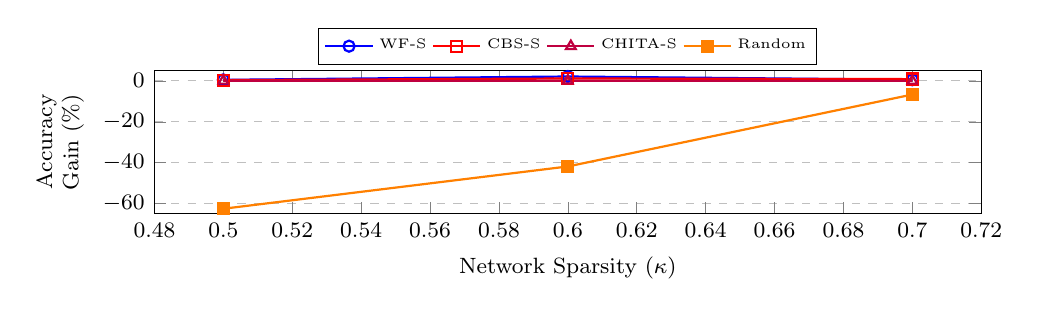
\begin{tikzpicture}
\begin{axis}[
    width=10.5cm,
    height=0.15\textwidth,
    scale only axis,
    xlabel={Network Sparsity (\(\kappa\))},
    ylabel={Accuracy \\ Gain (\%)},
    ylabel style={align=center},
    ymin=-65, ymax=5,
    ymajorgrids=true,
    grid style=dashed,
    legend pos=south east,
    legend style={
        at={(0.5,+1.3)},
        anchor=north,
        font=\tiny,
        cells={anchor=west},
        inner sep=2pt,
        legend columns=4,
    },
    tick label style={font=\footnotesize},
    label style={font=\footnotesize},
    legend cell align=left,
    mark options={scale=1},
    cycle list name=color list
]

\addplot[color=blue, mark=o, solid, thick] coordinates {
    (0.5, 0.49)
    (0.6, 2.13)
    (0.7, 0.55)
};
\addlegendentry{WF-S}

% CBS-S gain over MP
\addplot[color=red, mark=square, solid, thick] coordinates {
    (0.5, 0.35)
    (0.6, 1.16)
    (0.7, 0.85)
};
\addlegendentry{CBS-S}

% CHITA-S gain over MP
\addplot[color=purple, mark=triangle, solid, thick] coordinates {
    (0.5, 0.01)
    (0.6, 0.04)
    (0.7, 0.00)
};
\addlegendentry{CHITA-S}

\addplot[color=orange, mark=square*, solid, thick] coordinates {
    (0.5, -62.5)
    (0.6, -41.84)
    (0.7, -6.68)
};
\addlegendentry{Random}

\end{axis}
\end{tikzpicture}
\caption{Comparison of test accuracy gain over magnitude pruning for a pre-trained MobileNet (trained on ImageNet) at different sparsity levels.}
\label{fig:obs_selection}
\end{figure}


Further analysis of the similarity between pruning decisions made by MP and CHITA is provided in Appendix~\ref{appendix:pruning_similarity} to demonstrate that both methods produce nearly identical masks, underscoring the limited role of weight selection.



\subsection{Role of Hessian-Based Weight Updates}

While weight selection has negligible impact on accuracy, Hessian-based updates are critical for recovering accuracy by adjusting the remaining weights to compensate for accuracy loss due to pruning.

IP methods combine weight selection with Hessian-based updates (WF-U, CBS-U, CHITA-U). To evaluate the role of updates, we apply Hessian-based updates to MP and the resultant is denoted as MP-U. MP-U tests whether the benefits of Hessian-based updates generalize to MP's simpler selection strategy.
As shown in Figure~\ref{fig:obs_update}, MP-U achieves accuracy gains comparable to WF-U, CBS-U, and CHITA-U. This demonstrates that Hessian-based updates, not weight selection, is the primary driver of accuracy recovery. Combining Hessian-based updates with MP achieves performance on par with state-of-the-art pruning methods, eliminating the need for computationally expensive IP-selection strategies.





\begin{figure}[ht]
\centering
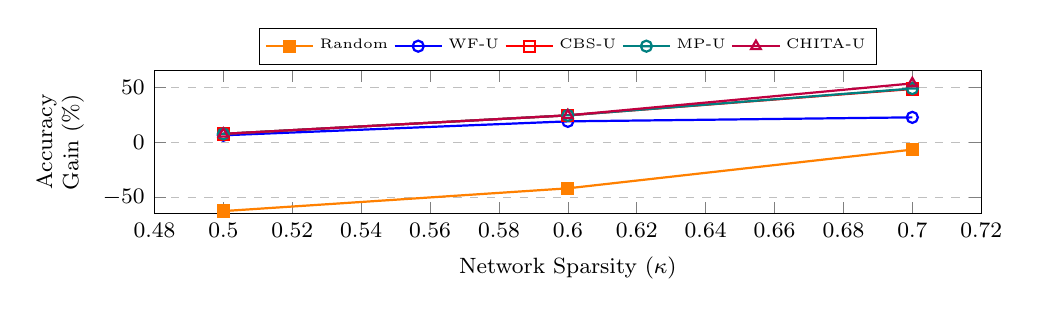
\begin{tikzpicture}
\begin{axis}[
    width=10.5cm,
    height=0.15\textwidth,
    scale only axis,
    xlabel={Network Sparsity (\(\kappa\))},
    ylabel={Accuracy \\ Gain (\%)},
    ylabel style={align=center},
    ymin=-65, ymax=65,
    ymajorgrids=true,
    grid style=dashed,
    legend pos=south east,
    legend style={
        at={(0.5,+1.3)},
        anchor=north,
        font=\tiny,
        cells={anchor=west},
        inner sep=2pt,
        legend columns=5,
    },
    tick label style={font=\footnotesize},
    label style={font=\footnotesize},
    legend cell align=left,
    mark options={scale=1},
    cycle list name=color list
]

\addplot[color=orange, mark=square*, solid, thick] coordinates {
    (0.5, -62.5)
    (0.6, -41.84)
    (0.7, -6.68)
};
\addlegendentry{Random}

\addplot[color=blue, mark=o, solid, thick] coordinates {
    (0.5, 6.3)
    (0.6, 18.96)
    (0.7, 22.58)
};
\addlegendentry{WF-U}

\addplot[color=red, mark=square, solid, thick] coordinates {
    (0.5, 7.6)
    (0.6, 24.43)
    (0.7, 48.33)
};
\addlegendentry{CBS-U}

\addplot[color=teal, mark=halfcircle, solid, thick] coordinates {
    (0.5, 7.63)
    (0.6, 24.39)
    (0.7, 48.73)
};
\addlegendentry{MP-U}


\addplot[color=purple, mark=triangle, solid, thick] coordinates {
    (0.5, 7.63)
    (0.6, 24.39)
    (0.7, 53.4)
};
\addlegendentry{CHITA-U}

\end{axis}
\end{tikzpicture}
\caption{Comparison of test accuracy gain over magnitude pruning for a pre-trained MobileNet (trained on ImageNet) at different sparsity levels.}
\label{fig:obs_update}
\end{figure}



\textbf{Insights}.
IP-selection only methods (WF-S, CBS-S, CHITA-S) offer minimal improvements over MP, confirming that weight selection has little influence on pruning performance. In contrast, Hessian-based update is the primary contributor to accuracy recovery post-pruning. These findings \textit{shift the focus from weight selection to identifying other factors affecting pruning performance}, which is explored in the next section.








\section{Understanding Signal Collapse and Restoring Performance Loss with REFLOW}
\label{sec:Signal_Propagation}
We examine the performance loss of pruned networks by introducing signal collapse - a phenomenon we observe for the first time, where one-shot pruning progressively reduces activation variance across layers, ultimately impairing the network’s ability to distinguish between inputs. In this section, we formally define signal collapse, explain its mechanisms, and demonstrate its impact on network performance. Finally, we introduce REFLOW, a method to mitigate signal collapse and restore the performance of one-shot pruned networks.
\subsection{Notation and Setup}

Consider a pre-trained neural network \( f(\theta) \), parameterized by \(\theta \in \mathbb{R}^d\). For a given layer \(\ell \in \{1, \dots, L\}\), let the input to layer \(\ell\) be denoted as \(\mathbf{H}_{\ell-1}\). The pre-BatchNorm (pre-BN) activation at layer \(\ell\) is defined as:
\begin{equation}
    \mathbf{X}_\ell = f(\mathbf{H}_{\ell-1}; \theta_\ell),
    \label{eq:pre_bn_signal_formal}
\end{equation}
where \(\theta_\ell\) represents the parameters of layer \(\ell\).

Batch Normalization (BN) normalizes the pre-BN activation \(\mathbf{X}_\ell\) across the batch as follows:
\begin{equation}
    \mathbf{Z}_\ell(n) = 
    \frac{\mathbf{X}_\ell(n) - \mu_\ell}
    {\sqrt{\mathrm{Var}_\ell^{\text{(Orig)}}(\mathbf{X}_\ell) + \epsilon}} \cdot \gamma_\ell + \beta_\ell,
    \label{eq:bn_transform}
\end{equation}
where \(n\) is the index of the batch dimension, \(\mu_\ell\) and \(\mathrm{Var}_\ell^{\text{(Orig)}}(\mathbf{X}_\ell)\) are the running mean and variance of the BN layer, \(\gamma_\ell\) and \(\beta_\ell\) are fixed affine parameters, and \(\epsilon > 0\) is a small constant for numerical stability.


\noindent \textbf{Defining Signal Collapse.}
\emph{Signal collapse} occurs in a pruned network if the variance of the activations reduces significantly in deeper layers compared to the original, unpruned network. Formally, let \(\mathrm{Var}_\ell^{(\text{Pruned})}\) and \(\mathrm{Var}_\ell^{(\text{Orig})}\) denote the variances of activations at layer \(\ell\) in the pruned and original networks, respectively. Signal collapse occurs if:
\begin{equation}
    \lim_{\ell \to L} 
    \frac{\mathrm{Var}_\ell^{(\text{Pruned})}}{\mathrm{Var}_\ell^{(\text{Orig})}}
    \;\to\; 0,
    \label{eq:signal_collapse_definition}
\end{equation}
where \(L\) is the total number of layers.

When the variance ratio approaches zero in deeper layers, the activations become nearly constant, resulting in a loss of distinction between inputs, causing uniform predictions.

\subsection{Why Pruning Causes Signal Collapse}
\label{subsec:mechanisms_signal_collapse}

Signal collapse arises due to two reasons explored below:

\paragraph{A) Activation variance reduces due to weight pruning}.

Pruning zeroes out weights based on a selection criterion, typically removing those with lower scores under the assumption that they contribute less to the network's performance. Formally, for layer \(\ell\), pruning modifies the weights \(\theta_\ell\) to \(\theta_\ell'\), where weights are set to zero if their score \(z_{i}\) falls below a threshold \(\tau\):
\begin{equation}
    W_{\ell,i}' = 
    \begin{cases}
        W_{\ell,i}, & \text{if } z_{i} > \tau \\
        0, & \text{otherwise}
    \end{cases},
    \label{eq:weight_pruning_general}
\end{equation}
where \(z_{i}\) represents the pruning score (e.g., magnitude, impact (loss) based heuristic, as discussed in Section \ref{sec:relatedwork}) for weight \(W_{\ell,i}\), and \(\tau\) is the pruning threshold determined by the desired sparsity level \(\kappa\).

To calculate the variance of the pre-BN activation after pruning, consider the activation in its pruned state:\begin{equation}
\mathbf{X}_\ell' = \sum_{i \in \mathcal{S}} W_{\ell,i}' H_{\ell-1,i},
\end{equation}
where \(\mathcal{S}\) is the set of non-pruned weights. Assuming that the activations \( H_{\ell-1,i} \) are independent and have a zero mean, the covariance terms between different \( H_{\ell-1,i} \) and \( H_{\ell-1,j} \) (for \( i \neq j \)) vanish. Therefore, the variance of \(\mathbf{X}_\ell'\) simplifies to:
\begin{equation}
    \mathrm{Var}_\ell^{\text{(Pruned)}}(\mathbf{X}_\ell') = \sum_{i \in \mathcal{S}} W_{\ell,i}'^2 \cdot \mathrm{Var}(H_{\ell-1,i}),
    \label{eq:pruned_variance}
\end{equation}

This leverages the property that the variance of a sum of independent random variables is the sum of their variances, and the scaling property \(\mathrm{Var}(aX) = a^2 \mathrm{Var}(X)\) for a constant \(a\).

Given that at high sparsity many weights are removed, especially those with lower scores, the sum in Equation~\ref{eq:pruned_variance} diminishes, leading to:
\begin{equation}
    \mathrm{Var}_\ell^{\text{(Pruned)}}(\mathbf{X}_\ell') \ll \mathrm{Var}_\ell^{\text{(Orig)}}(\mathbf{X}_\ell).
    \label{eq:variance_reduction}
\end{equation}
% This reduced variance is a direct consequence of pruning, as the removal of numerous low-scoring weights diminishes the diversity and scale of activations generated by each layer.

\paragraph{B) Over-Normalization due to BN mismatch}

As shown above, after one-shot pruning, pre-BN activations \(\mathbf{X}_\ell'\) have a lower variance, denoted as \(\mathrm{Var}_\ell^{\text{(Pruned)}}(\mathbf{X}_\ell')\). However, BN layers retain the original running statistics \((\mu_\ell, \mathrm{Var}_\ell^{\text{(Orig)}}(\mathbf{X}_\ell))\) computed prior to pruning. Consequently, the BN transformation for pruned activations is:
\begin{equation}
    \mathbf{Z}_\ell'(n) = 
    \frac{\mathbf{X}_\ell'(n) - \mu_\ell}
    {\sqrt{\mathrm{Var}_\ell^{\text{(Orig)}}(\mathbf{X}_\ell) + \epsilon}} \cdot \gamma_\ell + \beta_\ell.
    \label{eq:pruned_bn_variance}
\end{equation}
Here, both subtracting the mean \(\mu_\ell\) and adding  \(\beta_\ell\) do not affect the variance of $\mathbf{Z}_\ell'$, only the scaling factor \(\frac{\gamma_\ell}{\sqrt{\mathrm{Var}_\ell^{\text{(Orig)}}(\mathbf{X}_\ell) + \epsilon}}\) influences the variance of \(\mathbf{Z}_\ell'\).

Applying the property that \(\mathrm{Var}(aX) = a^2 \mathrm{Var}(X)\) for a constant \(a\), the variance of the post-BN activation becomes:
\begin{equation}
    \mathrm{Var}_\ell^{\text{(Pruned)}}(\mathbf{Z}_\ell') = \left( \frac{\gamma_\ell}{\sqrt{\mathrm{Var}_\ell^{\text{(Orig)}}(\mathbf{X}_\ell) + \epsilon}} \right)^2 \cdot \mathrm{Var}_\ell^{\text{(Pruned)}}(\mathbf{X}_\ell').
    \label{eq:var_z_pruned}
\end{equation}
Similarly, the variance of the original (unpruned) post-BN activation is:
\begin{equation}
    \mathrm{Var}_\ell^{\text{(Orig)}}(\mathbf{Z}_\ell) = \left( \frac{\gamma_\ell}{\sqrt{\mathrm{Var}_\ell^{\text{(Orig)}}(\mathbf{X}_\ell) + \epsilon}} \right)^2 \cdot \mathrm{Var}_\ell^{\text{(Orig)}}(\mathbf{X}_\ell).
    \label{eq:var_z_orig}
\end{equation}

Taking the ratio of the pruned to original post-BN variances:
\begin{equation}
    \frac{\mathrm{Var}_\ell^{\text{(Pruned)}}(\mathbf{Z}_\ell')}{\mathrm{Var}_\ell^{\text{(Orig)}}(\mathbf{Z}_\ell)} = \frac{\mathrm{Var}_\ell^{\text{(Pruned)}}(\mathbf{X}_\ell')}{\mathrm{Var}_\ell^{\text{(Orig)}}(\mathbf{X}_\ell)}.
    \label{eq:variance_ratio}
\end{equation}
Given that \(\mathrm{Var}_\ell^{\text{(Pruned)}}(\mathbf{X}_\ell') \ll \mathrm{Var}_\ell^{\text{(Orig)}}(\mathbf{X}_\ell)\) as established in Equation~\ref{eq:variance_reduction}, it follows that:
\begin{equation}
\mathrm{Var}_\ell^{\text{(Pruned)}}(\mathbf{Z}_\ell') \ll \mathrm{Var}_\ell^{\text{(Orig)}}(\mathbf{Z}_\ell).\label{eq:Z_diff}
\end{equation}
Thus, \textbf{Over-Normalization} causes post-BN activations to cluster closely around their mean, reducing their variance. 

\subsection{Cumulative Reduction in Activation Variance and Signal Collapse Across Layers}

Signal collapse arises because of the reduction in activation variance which \emph{cumulatively compounds} across deeper layers in the network. In this subsection, we analyze how this progressive decline emerges when considering post-BN outputs.

\noindent
\textbf{Scaling Factor \(\eta_\ell\).}
For each layer \(\ell\), define the \emph{variance scaling factor} \(\eta_\ell\) as:
\begin{equation}
    \eta_\ell 
    \;=\; 
    \frac{\mathrm{Var}_\ell^{\text{(Pruned)}}\!\bigl(\mathbf{Z}_\ell'\bigr)}
         {\mathrm{Var}_\ell^{\text{(Orig)}}\!\bigl(\mathbf{Z}_\ell\bigr)}
    \;<\; 1,
    \label{eq:scaling_factor}
\end{equation}
where \(\kappa \in [0,1]\) is the fraction of weights pruned. As \(\kappa \to 1\), more weights are removed, which generally makes \(\eta_\ell\) smaller via Equations \ref{eq:pruned_variance} and \ref{eq:Z_diff}.

\noindent
\textbf{Propagation of Variance Reduction.}
Because the \emph{input} to layer \(\ell+1\) is the \emph{post-BN} output of layer \(\ell\) (\(\mathbf{H}_{\ell+1} = \mathbf{Z}_\ell\)), the pruned input \(\mathbf{H}_{\ell+1}'\) is \(\mathbf{Z}_\ell'\). Consequently, any variance reduction at layer \(\ell\) affects layer \(\ell+1\), causing variance to shrink \emph{layer by layer} in the pruned network.

\noindent
\textbf{Cumulative Variance Scaling.}
Recursively applying Equation~\ref{eq:scaling_factor} across \(L\) layers, the cumulative variance scaling at the final layer $L$ becomes:
\begin{equation}
    \mathrm{Var}_L^{\text{(Pruned)}}\!\bigl(\mathbf{Z}_L'\bigr)
    \;=\;
    \Bigl(\,\prod_{\ell=1}^L \eta_\ell\Bigr)
    \,\mathrm{Var}_L^{\text{(Orig)}}\!\bigl(\mathbf{Z}_L\bigr).
    \label{eq:cumulative_variance}
\end{equation}
As an example consider the following. 
By assuming a modest constant per-layer scaling factor of \(\eta_\ell = 0.9\) across \(L = 25\) layers, the cumulative variance scaling becomes:
\begin{equation}
    \prod_{\ell=1}^{25} 0.9 = 0.9^{25} \approx 0.072.
    \label{eq:example_cumulative_variance}
\end{equation}


In practice, \(\eta_\ell\) varies across layers due to differences in sparsity distribution across layers, but the overall trend remains consistent: variance reduces as activations propagate through the pruned network. As \(\ell\) approaches \(L\), with increasing sparsity  \(\kappa\), 
\begin{equation}
    \;\;\lim_{\kappa \to 1}\;
    \mathrm{Var}_L^{\text{(Pruned)}}\bigl(\mathbf{Z}_L'\bigr)
    \;=\;
    \Bigl(\prod_{\ell=1}^L \eta_\ell\Bigr)\,
    \mathrm{Var}_L^{\text{(Orig)}}\!\bigl(\mathbf{Z}_L\bigr)
    \;\;\xrightarrow{}\;\;
    0,
    \label{eq:variance_approaching_zero}
\end{equation}
Consequently, the variance of the activations in the final layers approaches zero (see Figure~\ref{fig:variance_ratios}). 

\noindent
\textbf{Insight.}
Given that \(\mathrm{Var}_L^{\text{(Pruned)}}(\mathbf{Z}_L') \to 0\), the post-BN outputs converge to their mean (constant) value:
\begin{equation}
    \lim_{\mathrm{Var}(\mathbf{Z}_L') \to 0} 
    \;\mathbf{Z}_L'(n) 
    \;=\; 
    \mathrm{Mean}(\mathbf{Z}_L'(n))
    \label{eq:constant_activation}
\end{equation}
This implies that for any two distinct inputs \(\mathbf{x}_1\) and \(\mathbf{x}_2\),
$\mathbf{Z}_L'(\mathbf{x}_1) \approx \mathbf{Z}_L'(\mathbf{x}_2)$. We refer to this as \textit{signal collapse} (see Figure~\ref{fig:prediction_collapse}) and the network is incapable of distinguishing between inputs, thereby making it ineffective for downstream tasks, such as classification.





We empirically validate signal collapse using two \textbf{global scalar metrics} after each BN layer \(\ell\). These metrics summarize the behavior of normalized activations \(\mathbf{Z}_\ell\),


\begin{align}
    \mathrm{Mean}_\ell &= \frac{1}{|\mathbf{Z}_\ell|} \sum_{x \in \mathbf{Z}_\ell} x, \\
    \mathrm{Var}_\ell &= \frac{1}{|\mathbf{Z}_\ell|} \sum_{x \in \mathbf{Z}_\ell} \left( x - \mathrm{Mean}_\ell \right)^2.
\end{align}
where \(|\mathbf{Z}_\ell|\) denotes the total number of elements in the tensor \(\mathbf{Z}_\ell\). Figure~\ref{fig:variance_ratios} illustrates the signal variance ratio \(\frac{\mathrm{Var}_\ell^{\text{(Pruned)}}}{\mathrm{Var}_\ell^{\text{(Orig)}}}\) across layers at different sparsity levels \(\kappa\). The ratio progressively drops with increasing sparsity, remaining near 1 for 40\% sparsity, but drops below 0.1 after Layer~22 in 90\% sparsity, resulting in signal collapse.%, significantly compromising the network's ability to differentiate between inputs.


Figure~\ref{fig:prediction_collapse} demonstrates signal collapse in ResNet-20 on CIFAR-10. The unpruned model distributes predictions evenly across all classes in the test set. In contrast, at 90\% sparsity, the pruned network collapses, with over 99.4\% of inputs mapped to a single class. This behavior aligns with our analysis shown in Equation~\ref{eq:constant_activation}, leading to nearly identical representations for different inputs ($\mathbf{Z}'_L(\mathbf{x}_1) \approx \mathbf{Z}'_L(\mathbf{x}_2)$).


\begin{figure}[h]
\centering
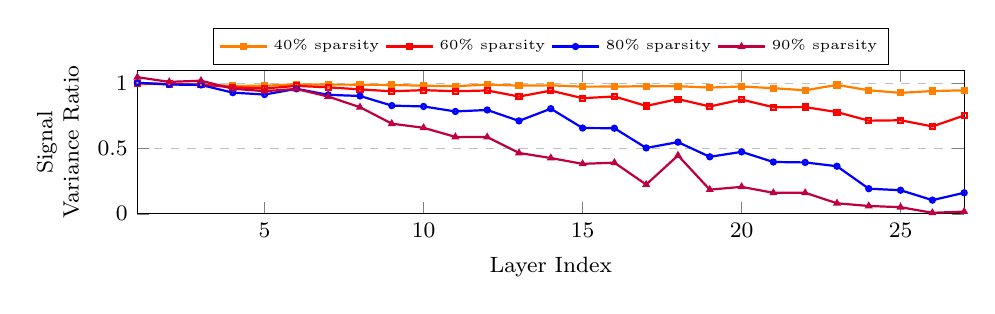
\begin{tikzpicture}
\begin{axis}[
    width=10.5cm,
    height=0.15\textwidth,
    scale only axis,
    xlabel={Layer Index},
    ylabel={Signal \\Variance Ratio},
    ylabel style={align=center},
    xmin=1, xmax=27,
    ymin=0, ymax=1.1,
    xtick={5,10,15,20,25},
    ymajorgrids=true,
    grid style=dashed,
    legend style={
        at={(0.5,+1.3)},
        anchor=north,
        font=\tiny,
        cells={anchor=west},
        inner sep=2pt,
        legend columns=4,
    },
    tick label style={font=\footnotesize},
    label style={font=\footnotesize},
    legend cell align=left,
    cycle list name=color list
]
% 40% sparsity
\addplot[color=orange, mark=square*, mark size=0.9pt, solid, thick] coordinates {
    (1,0.9982) (2,0.9968) (3,0.9934) (4,0.9820) (5,0.9844) (6,0.9947)
    (7,0.9928) (8,0.9922) (9,0.9898) (10,0.9843) (11,0.9805) (12,0.9928)
    (13,0.9851) (14,0.9870) (15,0.9771) (16,0.9775) (17,0.9806) (18,0.9806)
    (19,0.9700) (20,0.9784) (21,0.9651) (22,0.9490) (23,0.9904) (24,0.9490)
    (25,0.9293) (26,0.9433) (27,0.9487)
};

% 60% sparsity
\addplot[color=red, mark=square, mark size=0.9pt, solid, thick] coordinates {
    (1,1.0035) (2,0.9968) (3,0.9921) (4,0.9729) (5,0.9626) (6,0.9830) 
    (7,0.9717) (8,0.9561) (9,0.9413) (10,0.9502) (11,0.9416) (12,0.9476) 
    (13,0.9010) (14,0.9464) (15,0.8883) (16,0.9015) (17,0.8289) (18,0.8813) 
    (19,0.8248) (20,0.8777) (21,0.8190) (22,0.8200) (23,0.7814) (24,0.7156) 
    (25,0.7188) (26,0.6714) (27,0.7553)
};


% 80% sparsity
\addplot[color=blue, mark=o, mark size=0.9pt, solid, thick] coordinates {
    (1,1.0071) (2,0.9936) (3,0.9898) (4,0.9310) (5,0.9164) (6,0.9603) 
    (7,0.9142) (8,0.9054) (9,0.8313) (10,0.8248) (11,0.7865) (12,0.7979) 
    (13,0.7139) (14,0.8078) (15,0.6590) (16,0.6577) (17,0.5062) (18,0.5508) 
    (19,0.4380) (20,0.4762) (21,0.3983) (22,0.3949) (23,0.3657) (24,0.1931) 
    (25,0.1815) (26,0.1053) (27,0.1616)
};


% 90% sparsity
\addplot[color=purple, mark=triangle, mark size=0.9pt, solid, thick] coordinates {
    (1,1.0497) (2,1.0136) (3,1.0227) (4,0.9611) (5,0.9423) (6,0.9593)
    (7,0.9009) (8,0.8193) (9,0.6927) (10,0.6609) (11,0.5910) (12,0.5896)
    (13,0.4677) (14,0.4287) (15,0.3839) (16,0.3930) (17,0.2250) (18,0.4487)
    (19,0.1859) (20,0.2073) (21,0.1615) (22,0.1616) (23,0.0810) (24,0.0605)
    (25,0.0511) (26,0.0081) (27,0.0171)
};
\addlegendentry{40\% sparsity}
\addlegendentry{60\% sparsity}
\addlegendentry{80\% sparsity}
\addlegendentry{90\% sparsity}
\end{axis}
\end{tikzpicture}
\caption{Layer-wise signal variance ratios $
    \frac{\mathrm{Var}^{\text{(Pruned)}}}{\mathrm{Var}^{\text{(Orig)}}},
    \label{eq:variance_ratio}$ in pruned MobileNet (on ImageNet). Higher sparsity leads to severe signal collapse in deeper layers.}\label{fig:variance_ratios}
\end{figure}


\begin{figure}[t]
\centering
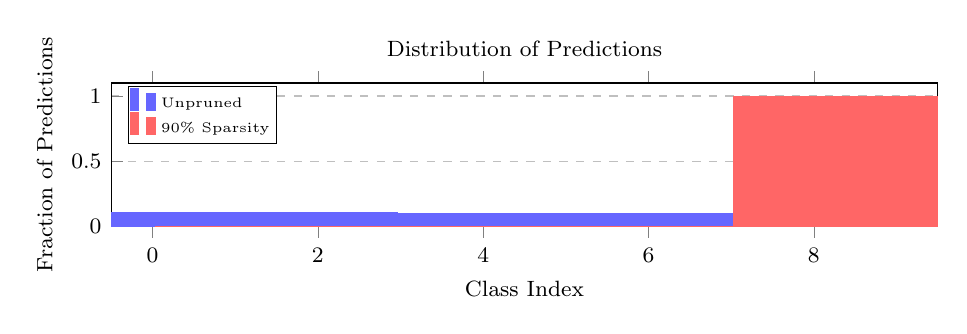
\begin{tikzpicture}
% Distribution Plot
\begin{axis}[
    width=10.5cm,
    height=0.15\textwidth,
    scale only axis,
    xlabel={Class Index},
    ylabel={Fraction of Predictions},
    xmin=-0.5, xmax=9.5,
    ymin=0, ymax=1.1,
    xtick={0,2,4,6,8},
    ymajorgrids=true,
    grid style=dashed,
    legend style={
        at={(0.02,0.98)},
        anchor=north west,
        font=\tiny,
        cells={anchor=west},
        inner sep=0.5pt,
        legend columns=1,
        scale=0.65,
        row sep=-2pt,
    },
    tick label style={font=\footnotesize},
    label style={font=\footnotesize},
    title={\footnotesize Distribution of Predictions},
    ybar,
    bar width=3,
]
% Original distribution
\addplot[blue!60, fill=blue!60] coordinates {
    (0,0.099600) (1,0.101300) (2,0.100100) (3,0.101500) (4,0.099300)
    (5,0.098900) (6,0.100600) (7,0.099900) (8,0.098700) (9,0.100100)
};
\addlegendentry{Unpruned}

% Updated 90% Pruned distribution
\addplot[red!60, fill=red!60] coordinates {
    (0,0.000000) (1,0.000000) (2,0.000500) (3,0.000000) (4,0.000000)
    (5,0.000000) (6,0.000000) (7,0.994800) (8,0.000000) (9,0.004700)
};
\addlegendentry{90\% Sparsity}
\end{axis}
\end{tikzpicture}
\caption{Distribution of predictions made by ResNet-20 on CIFAR-10. The unpruned model predicts uniformly across classes, discriminating between inputs, while the pruned model maps most inputs to a single class.}
\label{fig:prediction_collapse}
\end{figure}



\subsection{Hessian-Based Updates Mitigate but Do Not Fully Solve Signal Collapse}

Building on our earlier findings that Hessian-based updates are essential to recovering accuracy after pruning, we examine the effect of these updates on signal collapse. Specifically, we analyze how these updates influence the variance of activations across network layers.

\paragraph{Impact of Hessian-Based Updates on Signal Variance}

Figure~\ref{fig:variance_updates} presents the layer-wise signal variance ratios \(\frac{\mathrm{Var}_\ell^{\text{(Pruned)}}}{\mathrm{Var}_\ell^{\text{(Orig)}}}\) for three pruning methods: \textbf{CHITA-S} (selection-only), \textbf{MP-S} (Magnitude Pruning selection-only), and \textbf{CHITA-U} (selection with Hessian-based updates). 

As presented in Section~\ref{sec:revisiting_weight_selection}, \textbf{CHITA-S} and \textbf{MP-S} make near similar pruning decisions, resulting in identical (overlapping) variance profiles. Both pruning methods undergo signal collapse, with variance ratios frequently below 1 across layers. In contrast, \textbf{CHITA-U} maintains higher variance ratios in most layers, indicating that Hessian-based updates may help mitigate signal collapse. However, a few layers deeper in the network still show reduced variance ratios. This suggests that while Hessian-based updates reduce the impact of signal collapse, they do not entirely prevent it.

\begin{figure}[h]
\centering
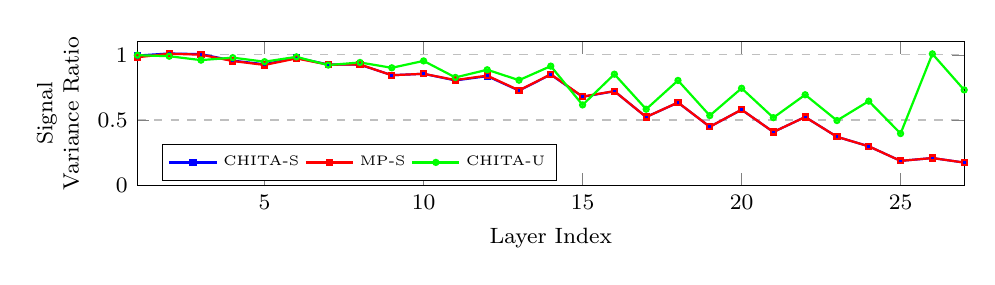
\begin{tikzpicture}
\begin{axis}[
    width=10.5cm,
    height=0.15\textwidth,
    scale only axis,
    xlabel={Layer Index},
    ylabel={Signal \\Variance Ratio},
    ylabel style={align=center},
    xmin=1, xmax=27,
    ymin=0, ymax=1.1,
    xtick={5,10,15,20,25},
    ymajorgrids=true,
    grid style=dashed,
    legend pos=south west,
    legend style={
        font=\tiny,
        cells={anchor=west},
        inner sep=2pt,
        legend columns=3,
    },
    tick label style={font=\footnotesize},
    label style={font=\footnotesize},
    legend cell align=left,
    cycle list name=color list
]
% CHITA-S
\addplot[color=blue, mark=square*, mark size=0.9pt, solid, thick] coordinates {
    (1,0.995) (2,1.011) (3,1.006) (4,0.956) (5,0.928) (6,0.978)
    (7,0.927) (8,0.925) (9,0.844) (10,0.855) (11,0.804) (12,0.837)
    (13,0.726) (14,0.849) (15,0.678) (16,0.721) (17,0.523) (18,0.634)
    (19,0.448) (20,0.579) (21,0.408) (22,0.523) (23,0.371) (24,0.298)
    (25,0.186) (26,0.208) (27,0.173)
};
% MP-S
\addplot[color=red, mark=square, mark size=0.9pt, solid, thick] coordinates {
    (1,0.982) (2,1.009) (3,1.002) (4,0.953) (5,0.923) (6,0.973)
    (7,0.925) (8,0.926) (9,0.844) (10,0.855) (11,0.807) (12,0.841)
    (13,0.728) (14,0.851) (15,0.680) (16,0.722) (17,0.523) (18,0.635)
    (19,0.448) (20,0.580) (21,0.408) (22,0.523) (23,0.371) (24,0.298)
    (25,0.186) (26,0.208) (27,0.173)
};
% CHITA-U
\addplot[color=green, mark=o, mark size=0.9pt, solid, thick] coordinates {
    (1,0.998) (2,0.990) (3,0.960) (4,0.979) (5,0.948) (6,0.985)
    (7,0.922) (8,0.942) (9,0.901) (10,0.954) (11,0.827) (12,0.886)
    (13,0.806) (14,0.914) (15,0.616) (16,0.852) (17,0.583) (18,0.804)
    (19,0.534) (20,0.744) (21,0.518) (22,0.694) (23,0.496) (24,0.645)
    (25,0.396) (26,1.008) (27,0.731)
};
\addlegendentry{CHITA-S}
\addlegendentry{MP-S}
\addlegendentry{CHITA-U}
\end{axis}
\end{tikzpicture}
\caption{Layer-wise signal variance ratios $\frac{\mathrm{Var}^{\text{(Pruned)}}}{\mathrm{Var}^{\text{(Baseline)}}}$ in 80\% sparse MobileNet on ImageNet. \textbf{CHITA-S} and \textbf{MP-S} show identical levels of signal collapse, while \textbf{CHITA-U} mitigates this collapse by Hessian-based updates.}\label{fig:variance_updates}
\end{figure}




\subsection{REFLOW: Restoring Signal Propagation to Mitigate Collapse}

\emph{Signal collapse} due to pruning stems from diminished activation variance. Hessian-based IP methods only partially mitigate signal collapse by updating the unpruned weights. These observations point to a more direct solution: if the core issue is the compounding mismatch between the pruned and original activation variances \(\frac{\mathrm{Var}_\ell^{\text{(Pruned)}}}{\mathrm{Var}_\ell^{\text{(Orig)}}} < 1\), resulting in signal collapse (Equation~\ref{eq:signal_collapse_definition}), then the running BN statistics can be calibrated to induce activation variance to mitigate signal collapse,  \emph{without} updating any unpruned (trainable) weights.


We propose \textbf{REFLOW} (\textbf{Re}storing \textbf{F}low of \textbf{Low}-variance signals), which updates only the BN running mean and variance after one-shot pruning. Specifically, rather than relying on the pre-pruning BN statistics $\bigl(\mu_\ell,\;\mathrm{Var}_\ell^{(\text{Orig})}\bigr)$, we collect a small calibration set $\mathcal{B}$ ($O(10)$ training batches) and pass it through the pruned network, and compute:
\begin{align}
\widehat{\mu}_\ell^{(\text{Pruned})}
  &= \frac{1}{|\mathcal{B}|} \sum_{n \in \mathcal{B}} \mathbf{X}_\ell'(n), \\
\widehat{\mathrm{Var}}_\ell^{(\text{Pruned})}(\mathbf{X}_\ell')
  &= \frac{1}{|\mathcal{B}|} \sum_{n \in \mathcal{B}}
    \Bigl(\mathbf{X}_\ell'(n) - \widehat{\mu}_\ell^{(\text{Pruned})}\Bigr)^2,
  \label{eq:reflow_calib}
\end{align}
where $\mathbf{X}_\ell'(n)$ are the pre-BN activations in the pruned model. We replace 
$\bigl(\mu_\ell,\;\mathrm{Var}_\ell^{(\text{Orig})}\bigr)$
with $\bigl(\widehat{\mu}_\ell^{(\text{Pruned})},\;\widehat{\mathrm{Var}}_\ell^{(\text{Pruned})}\bigr)$ in the BN layers, leaving $\gamma_\ell,\;\beta_\ell$ and all unpruned weights unchanged. The resulting post-BN activations become:
\begin{equation}
  \mathbf{Z}_\ell'^{(\text{REFLOW})}(n)
  \;=\;
  \frac{\mathbf{X}_\ell'(n) - \widehat{\mu}_\ell^{(\text{Pruned})}}
       {\sqrt{\widehat{\mathrm{Var}}_\ell^{(\text{Pruned})}(\mathbf{X}_\ell') + \epsilon}}
  \;\gamma_\ell \;+\; \beta_\ell.
  \label{eq:reflow_transform}
\end{equation}

\smallskip \noindent \textbf{Preserving Signal Variance}: REFLOW aligns each BN layer’s statistics with the \emph{true} statistics of the pruned pre-BN activations. This offsets the cumulative loss of variance that causes signal collapse. Figure~\ref{fig:reflow_effect}, shows recalibration at high sparsities restores the post-BN variance to the levels of the unpruned network. In doing so, REFLOW improves the network’s discriminative power by mitigating signal collapse without retraining or updating unpruned weights.




\begin{figure}[h]
\centering
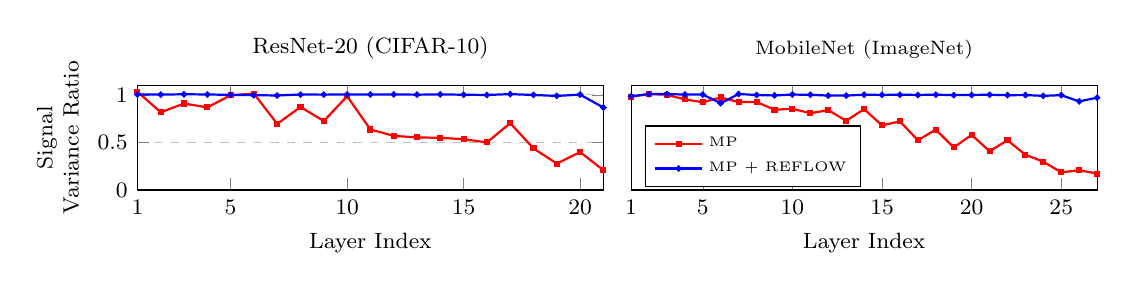
\begin{tikzpicture}
\begin{groupplot}[
    group style={
        group size=2 by 1,
        horizontal sep=10pt,
        vertical sep=0pt
    },
    width=7.5cm,
    height=0.24\textwidth,
    xlabel={Layer Index},
    xmin=1,
    ymin=0, ymax=1.1,
    ymajorgrids=true,
    grid style=dashed,
    tick label style={font=\footnotesize},
    label style={font=\footnotesize},
    legend cell align=left
]

%------------------ RESNET-20 ------------------%
\nextgroupplot[
    xmax=21,
    xtick={1,5,10,15,20},
    ylabel={Signal \\ Variance Ratio},
    ylabel style={align=center},
    title={\footnotesize ResNet-20 (CIFAR-10)}
]
\addplot[color=red, mark=square, mark size=0.7pt, solid, thick] coordinates {
(1,1.0345) (2,0.8172) (3,0.9096) (4,0.8688) (5,0.9972) (6,1.0141) (7,0.6961) (8,0.8730) (9,0.7257) (10,0.9861) (11,0.6367) (12,0.5695) (13,0.5532) (14,0.5492) (15,0.5341) (16,0.5009) (17,0.7034) (18,0.4376) (19,0.2782) (20,0.3987) (21,0.2088)};

\addplot[color=blue, mark=o, mark size=0.7pt, solid, thick] coordinates {
(1,1.0045) (2,1.0033) (3,1.0071) (4,1.0047) (5,1.0007) (6,0.9972) (7,0.9942) (8,1.0043) (9,1.0030) (10,1.0049) (11,1.0036) (12,1.0056) (13,1.0025) (14,1.0055) (15,1.0020) (16,0.9995) (17,1.0086) (18,0.9994) (19,0.9895) (20,1.0033) (21,0.8669)};

%------------------ MOBILENET ------------------%
\nextgroupplot[
    xmax=27,
    xtick={1,5,10,15,20,25},
    ytick = \empty,
    legend style={
        at={(0.03,0.03)},
        anchor=south west,
        font=\tiny,
        cells={anchor=west},
    },
    title={\scriptsize MobileNet (ImageNet)}
]
\addplot[color=red, mark=square, mark size=0.7pt, solid, thick] coordinates {
    (1,0.982) (2,1.009) (3,1.002) (4,0.953) (5,0.923) (6,0.973)
    (7,0.925) (8,0.926) (9,0.844) (10,0.855) (11,0.807) (12,0.841)
    (13,0.728) (14,0.851) (15,0.680) (16,0.722) (17,0.523) (18,0.635)
    (19,0.448) (20,0.580) (21,0.408) (22,0.523) (23,0.371) (24,0.298)
    (25,0.186) (26,0.208) (27,0.173)
};
\addlegendentry{MP}

\addplot[color=blue, mark=o, mark size=0.7pt, solid, thick] coordinates {
(1,0.9857) (2,1.0085) (3,1.0091) (4,1.0037) (5,1.0035) (6,0.9124) (7,1.0100) (8,0.9989) (9,0.9944) (10,1.0039) (11,1.0013) (12,0.9932) (13,0.9930) (14,1.0024) (15,1.0000) (16,1.0021) (17,1.0000) (18,1.0021) (19,0.9981) (20,1.0000) (21,1.0016) (22,0.9972) (23,0.9983) (24,0.9904) (25,0.9976) (26,0.9318) (27,0.9710)};
\addlegendentry{MP + REFLOW}

\end{groupplot}
\end{tikzpicture}

\caption{Layer-wise signal variance ratios in pruned networks under magnitude pruning at 80\% sparsity, before and after applying REFLOW.}
\label{fig:reflow_effect}
\end{figure}




\section{Experimental Results}
\label{sec:studies}
We apply REFLOW to magnitude pruning (MP) and evaluate it across small, medium, and large architectures. The results highlight REFLOW’s consistently recovers performance in pruned networks, achieving state-of-the-art accuracy without requiring computationally expensive Hessian-based updates. By mitigating signal collapse, REFLOW enables the discovery of high-quality sparse subnetworks within the original parameter space.

\subsection{Performance on Small Architectures}
We begin by evaluating REFLOW on small architectures, namely ResNet-20~\cite{RESNET} pre-trained on CIFAR-10~\cite{CIFAR10} and MobileNet~\cite{MobileNet} pre-trained on ImageNet~\cite{ImageNet}, with less than 5 million parameters and comparing them to state-of-the-art one-shot pruning approaches, namely WF~\cite{WoodFisher}, CBS~\cite{CBS}, and CHITA~\cite{CHITA}. 

Table~\ref{tab:small_architectures_results} highlights REFLOW’s accuracy improvements across all sparsity levels. For ResNet-20, REFLOW restores accuracy to 49.16\% at 0.9 sparsity, outperforming CHITA (15.60\%) and MP (11.79\%). On MobileNet, REFLOW achieves 43.37\% accuracy at 0.8 sparsity, surpassing CHITA (29.78\%) and MP (0.11\%). 

\begin{table}[h]
    \small
    \setlength{\tabcolsep}{4pt} % Reduce column padding
    \caption{Performance of pruning methods on small architectures (ResNet-20 on CIFAR-10 and MobileNet on ImageNet) across varying sparsity levels. Sparsity values represent the fraction of weights pruned (e.g., 0.4 corresponds to 40\% pruning). The unpruned test accuracy for ResNet-20 and MobileNet are 91.57\% and 71.96\%, respectively. The best accuracy values are highlighted in bold. Weight update indicates whether a single-pass Hessian-based update is performed on unpruned weights post-pruning.}
    \label{tab:small_architectures_results}
    \centering
    \resizebox{0.7\columnwidth}{!}{%
    \begin{tabular}{cccccccc}
        \toprule
        Dataset & Network & Sparsity & MP & WF & CBS & CHITA & REFLOW \\
        \midrule
        \multirow{6}{*}{CIFAR-10} & \multirow{6}{*}{ResNet-20} 
        & 0.4 & 89.98 & 91.15 & 91.21 & 91.19 & \textbf{91.25} \\
        & & 0.5 & 88.44 & 90.23 & 90.58 & 90.60 & \textbf{90.66} \\
        & & 0.6 & 85.24 & 87.96 & 88.88 & 89.22 & \textbf{89.49} \\
        & & 0.7 & 78.79 & 81.05 & 81.84 & 84.12 & \textbf{86.65} \\
        & & 0.8 & 54.01 & 62.63 & 51.28 & 57.90 & \textbf{78.50} \\
        & & 0.9 & 11.79 & 11.49 & 13.68 & 15.60 & \textbf{49.16} \\
        \midrule
        \multirow{5}{*}{ImageNet} & \multirow{5}{*}{MobileNet} 
        & 0.4 & 69.16 & 71.15 & 71.45 & 71.50 & \textbf{71.59} \\
        & & 0.5 & 62.61 & 68.91 & 70.21 & 70.42 & \textbf{70.48} \\
        & & 0.6 & 41.94 & 60.90 & 66.37 & 67.30 & \textbf{67.83} \\
        & & 0.7 & 6.78 & 29.36 & 55.11 & 59.40 & \textbf{61.54} \\
        & & 0.8 & 0.11 & 0.24 & 16.38 & 29.78 & \textbf{43.37} \\
        \midrule
        Weight Update & - & - &  \xmark & \cmark & \cmark & \cmark & \xmark \\
        \bottomrule
    \end{tabular}
    }
\end{table}

\subsection{Scaling REFLOW to Medium-sized Architectures}
We next evaluate REFLOW on medium-sized architectures, namely ResNet-50 (ImageNet) with less than 25 million parameters. For this size, we compare REFLOW to CHITA and M-FAC~\cite{mfac}, as WF and CBS are computationally prohibitive.

Figure~\ref{fig:resnet50_results} shows that REFLOW outperforms CHITA and M-FAC across all sparsity levels. At high sparsities, REFLOW offer superior accuracy improvements without the overhead of Hessian-based updates. %These results demonstrate that REFLOW’s mitigation of signal collapse scales effectively to larger models, maintaining both efficiency and high accuracy.
\begin{figure}[h]
    \centering
    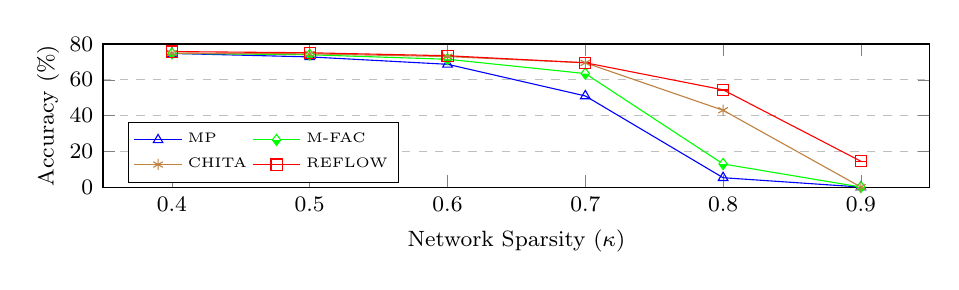
\begin{tikzpicture}
    \begin{axis}[
        width=10.5cm,
        height=0.15\textwidth,
        scale only axis,
        xlabel={Network Sparsity (\(\kappa\))},
        ylabel={Accuracy (\%)},
        xmin=0.35, xmax=0.95,
        ymin=0, ymax=80,
        ylabel near ticks,
        ylabel shift=-3pt,
        xtick={0.4,0.5,0.6,0.7,0.8,0.9},
        ymajorgrids=true,
        grid style=dashed,
        legend pos=south west,
        legend style={font=\tiny, cells={anchor=west}, inner sep=2pt, legend columns=2},
        tick label style={font=\footnotesize},
        label style={font=\footnotesize},
        legend cell align=left,
        mark options={scale=1},
        cycle list name=color list
    ]

    \addplot[color=blue,mark=triangle] coordinates {
        (0.40,74.74)
        (0.50,72.81) (0.60,68.68) 
        (0.70,51) (0.80,5.318) 
        (0.90,0.1)
    };
    \addlegendentry{MP}

    \addplot[color=green,mark=halfdiamond*] coordinates {
        (0.40,74.8)
        (0.50,74) (0.60,71.5) 
        (0.70,63.5) (0.80,13) 
        (0.90,0.1)
    };
    \addlegendentry{M-FAC}

    \addplot[color=brown,mark=asterisk] coordinates {
        (0.40,74.9)
        (0.50,74.5) (0.60,73) 
        (0.70,69.5) (0.80,43) 
        (0.90,0.1)
    };
    \addlegendentry{CHITA}

    \addplot[color=red,mark=square, error bars/.cd, y dir=both, y explicit] 
    coordinates {
        (0.40,75.788) +- (0,0.04)
        (0.50,75.12) +- (0,0.03)
        (0.60,73.466) +- (0,0.01)
        (0.70,69.55) +- (0,0.08)
        (0.80,54.412) +- (0,0.19)
        (0.90,14.506) +- (0,0.04)
    };
    \addlegendentry{REFLOW}

    \end{axis}
    \end{tikzpicture}
    \caption{Comparison of test accuracy for varying sparsities across pruning techniques for ResNet-50 on ImageNet. REFLOW outperforms CHITA, M-FAC, and MP consistently.}
    \label{fig:resnet50_results}
\end{figure}

\subsection{Scaling REFLOW to Large Architectures}
Finally, we consider large architectures, namely ResNet-101, ResNet-152, RegNetX-32GF (with nearly 107 million parameters), and ResNeXt-101 (64x4d) that has over 45 million parameters. These models pose significant challenges for pruning, particularly for CHITA as it relies on memory- and computation-intensive second-order approximations.
Figure~\ref{fig:large_architectures} shows that REFLOW delivers up to 74.8\% accuracy gains over MP on ImageNet. For instance, on ResNet-101, REFLOW restores accuracy from 4.1\% (MP) to 64.1\%. On ResNet-152, REFLOW achieves 68.2\% accuracy, compared to just 0.9\% for MP. Similar gains are observed for RegNetX-32GF, where REFLOW achieves 73.0\% accuracy, and for ResNeXt-101, where it achieves 78.9\%, outperforming MP. 

\begin{figure}[h]
    \centering
    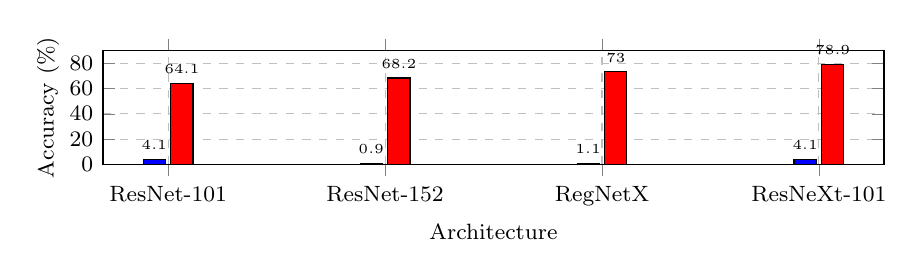
\begin{tikzpicture}
    \begin{axis}[
        width=11.5cm,
        height=0.25\textwidth,
        ybar,
        bar width=8pt,
        xlabel={Architecture},
        ylabel={\footnotesize Accuracy (\%)},
        ylabel style={font=\footnotesize}, % Apply tiny font to the ylabel
        ymin=0, ymax=90,
        xtick=data,
        xticklabel style={font=\footnotesize}, % Decreased font size for x-labels
        symbolic x coords={ResNet-101, ResNet-152, RegNetX, ResNeXt-101},
        grid=both,
        grid style=dashed,
        ymajorgrids=true,
        tick label style={font=\footnotesize}, % Set tick label font to tiny
        label style={font=\footnotesize}, % General label font size
        ylabel near ticks,
        ylabel shift=-3pt,
        legend style={font=\footnotesize, cells={anchor=west}, inner sep=2pt, legend columns=1, at={(0.5,1.05)}, anchor=south}, % Adjust legend style
        nodes near coords,
        every node near coord/.append style={font=\fontsize{0.1}{0.1}\selectfont} % Nodes near bars are tiny
    ]

    % MP Accuracy
    \addplot[fill=blue] coordinates {
        (ResNet-101, 4.1)
        (ResNet-152, 0.9)
        (RegNetX, 1.1)
        (ResNeXt-101, 4.1)
    };
    % \addlegendentry{MP}

    % REFLOW Accuracy
    \addplot[fill=red] coordinates {
        (ResNet-101, 64.1)
        (ResNet-152, 68.2)
        (RegNetX, 73.0)
        (ResNeXt-101, 78.9)
    };
    % \addlegendentry{REFLOW}

    \end{axis}
    \end{tikzpicture}
    \caption{Accuracy comparison of MP (blue) and REFLOW applied to MP (red) at 80\% sparsity for large architectures pre-trained on ImageNet. REFLOW mitigates signal collapse and restores accuracy.}
    \label{fig:large_architectures}
\end{figure}



\subsection{Convergence with REFLOW}
Building on the results in Table~\ref{tab:small_architectures_results}, we evaluate the impact of REFLOW across pruning methods with varying complexities: MP, CHITA-S (selection-only), and CHITA (selection with Hessian-based updates). CHITA updates the unpruned weights using second-order information, while CHITA-S applies the same selection criteria without weight updates. This distinction isolates the role of weight updates and quantifies whether REFLOW can compensate for their absence.

Figure~\ref{fig:reflow_convergence} shows that REFLOW bridges the performance gap between MP, CHITA-S, and CHITA. REFLOW enables simpler selection based approaches like MP and CHITA-S to achieve comparable accuracy as CHITA (Hessian-based weight updates) although the latter is computationally intensive. This highlights that mitigating signal collapse, rather than employing complex pruning selection heuristics, is the key to recovering performance in one-shot pruned networks.




\begin{figure}[h]
    \centering
    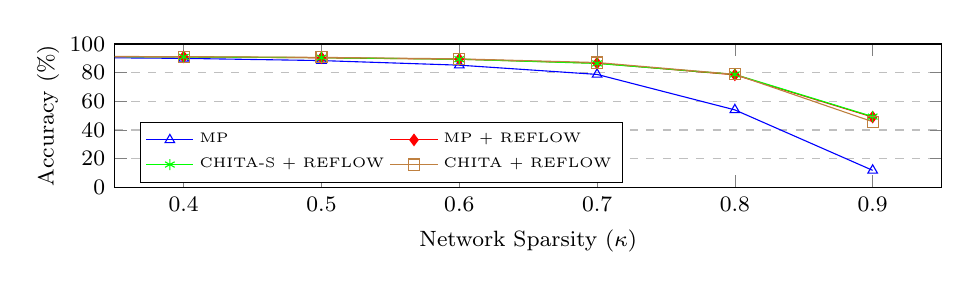
\begin{tikzpicture}
    \begin{axis}[
        width=10.5cm,
        height=0.15\textwidth,
        scale only axis,
        xlabel={Network Sparsity (\(\kappa\))},
        ylabel={Accuracy (\%)},
        xmin=0.35, xmax=0.95,
        ymin=0, ymax=100,
        ylabel near ticks,
        ylabel shift=-3pt,
        xtick={0.4,0.5,0.6,0.7,0.8,0.9},
        ymajorgrids=true,
        grid style=dashed,
        legend pos=south west,
        legend style={font=\tiny, cells={anchor=west}, inner sep=2pt, legend columns=2},
        tick label style={font=\footnotesize},
        label style={font=\footnotesize},
        legend cell align=left,
        mark options={scale=1},
        cycle list name=color list
    ]

    % MP (Blue)
    \addplot[color=blue,mark=triangle] coordinates {
        (0.3,90.77) (0.4,89.98) (0.5,88.44) 
        (0.6,85.24) (0.7,78.79) (0.8,54.01) 
        (0.9,11.79)
    };
    \addlegendentry{MP}

    % MP + REFLOW (Red)
    \addplot[color=red,mark=diamond*] coordinates {
        (0.3,91.41) (0.4,91.05) (0.5,90.39) 
        (0.6,89.38) (0.7,86.65) (0.8,78.5) 
        (0.9,49.0)
    };
    \addlegendentry{MP + REFLOW}

    % CHITA-S + REFLOW (Green)
    \addplot[color=green,mark=asterisk] coordinates {
        (0.3,91.37) (0.4,91.0) (0.5,90.45) 
        (0.6,89.41) (0.7,86.45) (0.8,78.79) 
        (0.9,49.35)
    };
    \addlegendentry{CHITA-S + REFLOW}

    % CHITA-U + REFLOW (Brown)
    \addplot[color=brown,mark=square, error bars/.cd, y dir=both, y explicit] 
    coordinates {
        (0.3,91.43) (0.4,91.17) (0.5,90.68) 
        (0.6,89.64) (0.7,87.08) (0.8,78.84) 
        (0.9,45.76)
    };
    \addlegendentry{CHITA + REFLOW}

    \end{axis}
    \end{tikzpicture}
    \caption{Comparison of test accuracy vs. sparsity for ResNet-20 on CIFAR-10.}
    \label{fig:reflow_convergence}
\end{figure}






\section{Conclusion}
\label{sec:discussion}
\section{Discussion of Assumptions}\label{sec:discussion}
In this paper, we have made several assumptions for the sake of clarity and simplicity. In this section, we discuss the rationale behind these assumptions, the extent to which these assumptions hold in practice, and the consequences for our protocol when these assumptions hold.

\subsection{Assumptions on the Demand}

There are two simplifying assumptions we make about the demand. First, we assume the demand at any time is relatively small compared to the channel capacities. Second, we take the demand to be constant over time. We elaborate upon both these points below.

\paragraph{Small demands} The assumption that demands are small relative to channel capacities is made precise in \eqref{eq:large_capacity_assumption}. This assumption simplifies two major aspects of our protocol. First, it largely removes congestion from consideration. In \eqref{eq:primal_problem}, there is no constraint ensuring that total flow in both directions stays below capacity--this is always met. Consequently, there is no Lagrange multiplier for congestion and no congestion pricing; only imbalance penalties apply. In contrast, protocols in \cite{sivaraman2020high, varma2021throughput, wang2024fence} include congestion fees due to explicit congestion constraints. Second, the bound \eqref{eq:large_capacity_assumption} ensures that as long as channels remain balanced, the network can always meet demand, no matter how the demand is routed. Since channels can rebalance when necessary, they never drop transactions. This allows prices and flows to adjust as per the equations in \eqref{eq:algorithm}, which makes it easier to prove the protocol's convergence guarantees. This also preserves the key property that a channel's price remains proportional to net money flow through it.

In practice, payment channel networks are used most often for micro-payments, for which on-chain transactions are prohibitively expensive; large transactions typically take place directly on the blockchain. For example, according to \cite{river2023lightning}, the average channel capacity is roughly $0.1$ BTC ($5,000$ BTC distributed over $50,000$ channels), while the average transaction amount is less than $0.0004$ BTC ($44.7k$ satoshis). Thus, the small demand assumption is not too unrealistic. Additionally, the occasional large transaction can be treated as a sequence of smaller transactions by breaking it into packets and executing each packet serially (as done by \cite{sivaraman2020high}).
Lastly, a good path discovery process that favors large capacity channels over small capacity ones can help ensure that the bound in \eqref{eq:large_capacity_assumption} holds.

\paragraph{Constant demands} 
In this work, we assume that any transacting pair of nodes have a steady transaction demand between them (see Section \ref{sec:transaction_requests}). Making this assumption is necessary to obtain the kind of guarantees that we have presented in this paper. Unless the demand is steady, it is unreasonable to expect that the flows converge to a steady value. Weaker assumptions on the demand lead to weaker guarantees. For example, with the more general setting of stochastic, but i.i.d. demand between any two nodes, \cite{varma2021throughput} shows that the channel queue lengths are bounded in expectation. If the demand can be arbitrary, then it is very hard to get any meaningful performance guarantees; \cite{wang2024fence} shows that even for a single bidirectional channel, the competitive ratio is infinite. Indeed, because a PCN is a decentralized system and decisions must be made based on local information alone, it is difficult for the network to find the optimal detailed balance flow at every time step with a time-varying demand.  With a steady demand, the network can discover the optimal flows in a reasonably short time, as our work shows.

We view the constant demand assumption as an approximation for a more general demand process that could be piece-wise constant, stochastic, or both (see simulations in Figure \ref{fig:five_nodes_variable_demand}).
We believe it should be possible to merge ideas from our work and \cite{varma2021throughput} to provide guarantees in a setting with random demands with arbitrary means. We leave this for future work. In addition, our work suggests that a reasonable method of handling stochastic demands is to queue the transaction requests \textit{at the source node} itself. This queuing action should be viewed in conjunction with flow-control. Indeed, a temporarily high unidirectional demand would raise prices for the sender, incentivizing the sender to stop sending the transactions. If the sender queues the transactions, they can send them later when prices drop. This form of queuing does not require any overhaul of the basic PCN infrastructure and is therefore simpler to implement than per-channel queues as suggested by \cite{sivaraman2020high} and \cite{varma2021throughput}.

\subsection{The Incentive of Channels}
The actions of the channels as prescribed by the DEBT control protocol can be summarized as follows. Channels adjust their prices in proportion to the net flow through them. They rebalance themselves whenever necessary and execute any transaction request that has been made of them. We discuss both these aspects below.

\paragraph{On Prices}
In this work, the exclusive role of channel prices is to ensure that the flows through each channel remains balanced. In practice, it would be important to include other components in a channel's price/fee as well: a congestion price  and an incentive price. The congestion price, as suggested by \cite{varma2021throughput}, would depend on the total flow of transactions through the channel, and would incentivize nodes to balance the load over different paths. The incentive price, which is commonly used in practice \cite{river2023lightning}, is necessary to provide channels with an incentive to serve as an intermediary for different channels. In practice, we expect both these components to be smaller than the imbalance price. Consequently, we expect the behavior of our protocol to be similar to our theoretical results even with these additional prices.

A key aspect of our protocol is that channel fees are allowed to be negative. Although the original Lightning network whitepaper \cite{poon2016bitcoin} suggests that negative channel prices may be a good solution to promote rebalancing, the idea of negative prices in not very popular in the literature. To our knowledge, the only prior work with this feature is \cite{varma2021throughput}. Indeed, in papers such as \cite{van2021merchant} and \cite{wang2024fence}, the price function is explicitly modified such that the channel price is never negative. The results of our paper show the benefits of negative prices. For one, in steady state, equal flows in both directions ensure that a channel doesn't loose any money (the other price components mentioned above ensure that the channel will only gain money). More importantly, negative prices are important to ensure that the protocol selectively stifles acyclic flows while allowing circulations to flow. Indeed, in the example of Section \ref{sec:flow_control_example}, the flows between nodes $A$ and $C$ are left on only because the large positive price over one channel is canceled by the corresponding negative price over the other channel, leading to a net zero price.

Lastly, observe that in the DEBT control protocol, the price charged by a channel does not depend on its capacity. This is a natural consequence of the price being the Lagrange multiplier for the net-zero flow constraint, which also does not depend on the channel capacity. In contrast, in many other works, the imbalance price is normalized by the channel capacity \cite{ren2018optimal, lin2020funds, wang2024fence}; this is shown to work well in practice. The rationale for such a price structure is explained well in \cite{wang2024fence}, where this fee is derived with the aim of always maintaining some balance (liquidity) at each end of every channel. This is a reasonable aim if a channel is to never rebalance itself; the experiments of the aforementioned papers are conducted in such a regime. In this work, however, we allow the channels to rebalance themselves a few times in order to settle on a detailed balance flow. This is because our focus is on the long-term steady state performance of the protocol. This difference in perspective also shows up in how the price depends on the channel imbalance. \cite{lin2020funds} and \cite{wang2024fence} advocate for strictly convex prices whereas this work and \cite{varma2021throughput} propose linear prices.

\paragraph{On Rebalancing} 
Recall that the DEBT control protocol ensures that the flows in the network converge to a detailed balance flow, which can be sustained perpetually without any rebalancing. However, during the transient phase (before convergence), channels may have to perform on-chain rebalancing a few times. Since rebalancing is an expensive operation, it is worthwhile discussing methods by which channels can reduce the extent of rebalancing. One option for the channels to reduce the extent of rebalancing is to increase their capacity; however, this comes at the cost of locking in more capital. Each channel can decide for itself the optimum amount of capital to lock in. Another option, which we discuss in Section \ref{sec:five_node}, is for channels to increase the rate $\gamma$ at which they adjust prices. 

Ultimately, whether or not it is beneficial for a channel to rebalance depends on the time-horizon under consideration. Our protocol is based on the assumption that the demand remains steady for a long period of time. If this is indeed the case, it would be worthwhile for a channel to rebalance itself as it can make up this cost through the incentive fees gained from the flow of transactions through it in steady state. If a channel chooses not to rebalance itself, however, there is a risk of being trapped in a deadlock, which is suboptimal for not only the nodes but also the channel.

\section{Conclusion}
This work presents DEBT control: a protocol for payment channel networks that uses source routing and flow control based on channel prices. The protocol is derived by posing a network utility maximization problem and analyzing its dual minimization. It is shown that under steady demands, the protocol guides the network to an optimal, sustainable point. Simulations show its robustness to demand variations. The work demonstrates that simple protocols with strong theoretical guarantees are possible for PCNs and we hope it inspires further theoretical research in this direction.




\bibliographystyle{plainnat}
\bibliography{Main}


\newpage
\appendix
\onecolumn
\subsection{Lloyd-Max Algorithm}
\label{subsec:Lloyd-Max}
For a given quantization bitwidth $B$ and an operand $\bm{X}$, the Lloyd-Max algorithm finds $2^B$ quantization levels $\{\hat{x}_i\}_{i=1}^{2^B}$ such that quantizing $\bm{X}$ by rounding each scalar in $\bm{X}$ to the nearest quantization level minimizes the quantization MSE. 

The algorithm starts with an initial guess of quantization levels and then iteratively computes quantization thresholds $\{\tau_i\}_{i=1}^{2^B-1}$ and updates quantization levels $\{\hat{x}_i\}_{i=1}^{2^B}$. Specifically, at iteration $n$, thresholds are set to the midpoints of the previous iteration's levels:
\begin{align*}
    \tau_i^{(n)}=\frac{\hat{x}_i^{(n-1)}+\hat{x}_{i+1}^{(n-1)}}2 \text{ for } i=1\ldots 2^B-1
\end{align*}
Subsequently, the quantization levels are re-computed as conditional means of the data regions defined by the new thresholds:
\begin{align*}
    \hat{x}_i^{(n)}=\mathbb{E}\left[ \bm{X} \big| \bm{X}\in [\tau_{i-1}^{(n)},\tau_i^{(n)}] \right] \text{ for } i=1\ldots 2^B
\end{align*}
where to satisfy boundary conditions we have $\tau_0=-\infty$ and $\tau_{2^B}=\infty$. The algorithm iterates the above steps until convergence.

Figure \ref{fig:lm_quant} compares the quantization levels of a $7$-bit floating point (E3M3) quantizer (left) to a $7$-bit Lloyd-Max quantizer (right) when quantizing a layer of weights from the GPT3-126M model at a per-tensor granularity. As shown, the Lloyd-Max quantizer achieves substantially lower quantization MSE. Further, Table \ref{tab:FP7_vs_LM7} shows the superior perplexity achieved by Lloyd-Max quantizers for bitwidths of $7$, $6$ and $5$. The difference between the quantizers is clear at 5 bits, where per-tensor FP quantization incurs a drastic and unacceptable increase in perplexity, while Lloyd-Max quantization incurs a much smaller increase. Nevertheless, we note that even the optimal Lloyd-Max quantizer incurs a notable ($\sim 1.5$) increase in perplexity due to the coarse granularity of quantization. 

\begin{figure}[h]
  \centering
  \includegraphics[width=0.7\linewidth]{sections/figures/LM7_FP7.pdf}
  \caption{\small Quantization levels and the corresponding quantization MSE of Floating Point (left) vs Lloyd-Max (right) Quantizers for a layer of weights in the GPT3-126M model.}
  \label{fig:lm_quant}
\end{figure}

\begin{table}[h]\scriptsize
\begin{center}
\caption{\label{tab:FP7_vs_LM7} \small Comparing perplexity (lower is better) achieved by floating point quantizers and Lloyd-Max quantizers on a GPT3-126M model for the Wikitext-103 dataset.}
\begin{tabular}{c|cc|c}
\hline
 \multirow{2}{*}{\textbf{Bitwidth}} & \multicolumn{2}{|c|}{\textbf{Floating-Point Quantizer}} & \textbf{Lloyd-Max Quantizer} \\
 & Best Format & Wikitext-103 Perplexity & Wikitext-103 Perplexity \\
\hline
7 & E3M3 & 18.32 & 18.27 \\
6 & E3M2 & 19.07 & 18.51 \\
5 & E4M0 & 43.89 & 19.71 \\
\hline
\end{tabular}
\end{center}
\end{table}

\subsection{Proof of Local Optimality of LO-BCQ}
\label{subsec:lobcq_opt_proof}
For a given block $\bm{b}_j$, the quantization MSE during LO-BCQ can be empirically evaluated as $\frac{1}{L_b}\lVert \bm{b}_j- \bm{\hat{b}}_j\rVert^2_2$ where $\bm{\hat{b}}_j$ is computed from equation (\ref{eq:clustered_quantization_definition}) as $C_{f(\bm{b}_j)}(\bm{b}_j)$. Further, for a given block cluster $\mathcal{B}_i$, we compute the quantization MSE as $\frac{1}{|\mathcal{B}_{i}|}\sum_{\bm{b} \in \mathcal{B}_{i}} \frac{1}{L_b}\lVert \bm{b}- C_i^{(n)}(\bm{b})\rVert^2_2$. Therefore, at the end of iteration $n$, we evaluate the overall quantization MSE $J^{(n)}$ for a given operand $\bm{X}$ composed of $N_c$ block clusters as:
\begin{align*}
    \label{eq:mse_iter_n}
    J^{(n)} = \frac{1}{N_c} \sum_{i=1}^{N_c} \frac{1}{|\mathcal{B}_{i}^{(n)}|}\sum_{\bm{v} \in \mathcal{B}_{i}^{(n)}} \frac{1}{L_b}\lVert \bm{b}- B_i^{(n)}(\bm{b})\rVert^2_2
\end{align*}

At the end of iteration $n$, the codebooks are updated from $\mathcal{C}^{(n-1)}$ to $\mathcal{C}^{(n)}$. However, the mapping of a given vector $\bm{b}_j$ to quantizers $\mathcal{C}^{(n)}$ remains as  $f^{(n)}(\bm{b}_j)$. At the next iteration, during the vector clustering step, $f^{(n+1)}(\bm{b}_j)$ finds new mapping of $\bm{b}_j$ to updated codebooks $\mathcal{C}^{(n)}$ such that the quantization MSE over the candidate codebooks is minimized. Therefore, we obtain the following result for $\bm{b}_j$:
\begin{align*}
\frac{1}{L_b}\lVert \bm{b}_j - C_{f^{(n+1)}(\bm{b}_j)}^{(n)}(\bm{b}_j)\rVert^2_2 \le \frac{1}{L_b}\lVert \bm{b}_j - C_{f^{(n)}(\bm{b}_j)}^{(n)}(\bm{b}_j)\rVert^2_2
\end{align*}

That is, quantizing $\bm{b}_j$ at the end of the block clustering step of iteration $n+1$ results in lower quantization MSE compared to quantizing at the end of iteration $n$. Since this is true for all $\bm{b} \in \bm{X}$, we assert the following:
\begin{equation}
\begin{split}
\label{eq:mse_ineq_1}
    \tilde{J}^{(n+1)} &= \frac{1}{N_c} \sum_{i=1}^{N_c} \frac{1}{|\mathcal{B}_{i}^{(n+1)}|}\sum_{\bm{b} \in \mathcal{B}_{i}^{(n+1)}} \frac{1}{L_b}\lVert \bm{b} - C_i^{(n)}(b)\rVert^2_2 \le J^{(n)}
\end{split}
\end{equation}
where $\tilde{J}^{(n+1)}$ is the the quantization MSE after the vector clustering step at iteration $n+1$.

Next, during the codebook update step (\ref{eq:quantizers_update}) at iteration $n+1$, the per-cluster codebooks $\mathcal{C}^{(n)}$ are updated to $\mathcal{C}^{(n+1)}$ by invoking the Lloyd-Max algorithm \citep{Lloyd}. We know that for any given value distribution, the Lloyd-Max algorithm minimizes the quantization MSE. Therefore, for a given vector cluster $\mathcal{B}_i$ we obtain the following result:

\begin{equation}
    \frac{1}{|\mathcal{B}_{i}^{(n+1)}|}\sum_{\bm{b} \in \mathcal{B}_{i}^{(n+1)}} \frac{1}{L_b}\lVert \bm{b}- C_i^{(n+1)}(\bm{b})\rVert^2_2 \le \frac{1}{|\mathcal{B}_{i}^{(n+1)}|}\sum_{\bm{b} \in \mathcal{B}_{i}^{(n+1)}} \frac{1}{L_b}\lVert \bm{b}- C_i^{(n)}(\bm{b})\rVert^2_2
\end{equation}

The above equation states that quantizing the given block cluster $\mathcal{B}_i$ after updating the associated codebook from $C_i^{(n)}$ to $C_i^{(n+1)}$ results in lower quantization MSE. Since this is true for all the block clusters, we derive the following result: 
\begin{equation}
\begin{split}
\label{eq:mse_ineq_2}
     J^{(n+1)} &= \frac{1}{N_c} \sum_{i=1}^{N_c} \frac{1}{|\mathcal{B}_{i}^{(n+1)}|}\sum_{\bm{b} \in \mathcal{B}_{i}^{(n+1)}} \frac{1}{L_b}\lVert \bm{b}- C_i^{(n+1)}(\bm{b})\rVert^2_2  \le \tilde{J}^{(n+1)}   
\end{split}
\end{equation}

Following (\ref{eq:mse_ineq_1}) and (\ref{eq:mse_ineq_2}), we find that the quantization MSE is non-increasing for each iteration, that is, $J^{(1)} \ge J^{(2)} \ge J^{(3)} \ge \ldots \ge J^{(M)}$ where $M$ is the maximum number of iterations. 
%Therefore, we can say that if the algorithm converges, then it must be that it has converged to a local minimum. 
\hfill $\blacksquare$


\begin{figure}
    \begin{center}
    \includegraphics[width=0.5\textwidth]{sections//figures/mse_vs_iter.pdf}
    \end{center}
    \caption{\small NMSE vs iterations during LO-BCQ compared to other block quantization proposals}
    \label{fig:nmse_vs_iter}
\end{figure}

Figure \ref{fig:nmse_vs_iter} shows the empirical convergence of LO-BCQ across several block lengths and number of codebooks. Also, the MSE achieved by LO-BCQ is compared to baselines such as MXFP and VSQ. As shown, LO-BCQ converges to a lower MSE than the baselines. Further, we achieve better convergence for larger number of codebooks ($N_c$) and for a smaller block length ($L_b$), both of which increase the bitwidth of BCQ (see Eq \ref{eq:bitwidth_bcq}).


\subsection{Additional Accuracy Results}
%Table \ref{tab:lobcq_config} lists the various LOBCQ configurations and their corresponding bitwidths.
\begin{table}
\setlength{\tabcolsep}{4.75pt}
\begin{center}
\caption{\label{tab:lobcq_config} Various LO-BCQ configurations and their bitwidths.}
\begin{tabular}{|c||c|c|c|c||c|c||c|} 
\hline
 & \multicolumn{4}{|c||}{$L_b=8$} & \multicolumn{2}{|c||}{$L_b=4$} & $L_b=2$ \\
 \hline
 \backslashbox{$L_A$\kern-1em}{\kern-1em$N_c$} & 2 & 4 & 8 & 16 & 2 & 4 & 2 \\
 \hline
 64 & 4.25 & 4.375 & 4.5 & 4.625 & 4.375 & 4.625 & 4.625\\
 \hline
 32 & 4.375 & 4.5 & 4.625& 4.75 & 4.5 & 4.75 & 4.75 \\
 \hline
 16 & 4.625 & 4.75& 4.875 & 5 & 4.75 & 5 & 5 \\
 \hline
\end{tabular}
\end{center}
\end{table}

%\subsection{Perplexity achieved by various LO-BCQ configurations on Wikitext-103 dataset}

\begin{table} \centering
\begin{tabular}{|c||c|c|c|c||c|c||c|} 
\hline
 $L_b \rightarrow$& \multicolumn{4}{c||}{8} & \multicolumn{2}{c||}{4} & 2\\
 \hline
 \backslashbox{$L_A$\kern-1em}{\kern-1em$N_c$} & 2 & 4 & 8 & 16 & 2 & 4 & 2  \\
 %$N_c \rightarrow$ & 2 & 4 & 8 & 16 & 2 & 4 & 2 \\
 \hline
 \hline
 \multicolumn{8}{c}{GPT3-1.3B (FP32 PPL = 9.98)} \\ 
 \hline
 \hline
 64 & 10.40 & 10.23 & 10.17 & 10.15 &  10.28 & 10.18 & 10.19 \\
 \hline
 32 & 10.25 & 10.20 & 10.15 & 10.12 &  10.23 & 10.17 & 10.17 \\
 \hline
 16 & 10.22 & 10.16 & 10.10 & 10.09 &  10.21 & 10.14 & 10.16 \\
 \hline
  \hline
 \multicolumn{8}{c}{GPT3-8B (FP32 PPL = 7.38)} \\ 
 \hline
 \hline
 64 & 7.61 & 7.52 & 7.48 &  7.47 &  7.55 &  7.49 & 7.50 \\
 \hline
 32 & 7.52 & 7.50 & 7.46 &  7.45 &  7.52 &  7.48 & 7.48  \\
 \hline
 16 & 7.51 & 7.48 & 7.44 &  7.44 &  7.51 &  7.49 & 7.47  \\
 \hline
\end{tabular}
\caption{\label{tab:ppl_gpt3_abalation} Wikitext-103 perplexity across GPT3-1.3B and 8B models.}
\end{table}

\begin{table} \centering
\begin{tabular}{|c||c|c|c|c||} 
\hline
 $L_b \rightarrow$& \multicolumn{4}{c||}{8}\\
 \hline
 \backslashbox{$L_A$\kern-1em}{\kern-1em$N_c$} & 2 & 4 & 8 & 16 \\
 %$N_c \rightarrow$ & 2 & 4 & 8 & 16 & 2 & 4 & 2 \\
 \hline
 \hline
 \multicolumn{5}{|c|}{Llama2-7B (FP32 PPL = 5.06)} \\ 
 \hline
 \hline
 64 & 5.31 & 5.26 & 5.19 & 5.18  \\
 \hline
 32 & 5.23 & 5.25 & 5.18 & 5.15  \\
 \hline
 16 & 5.23 & 5.19 & 5.16 & 5.14  \\
 \hline
 \multicolumn{5}{|c|}{Nemotron4-15B (FP32 PPL = 5.87)} \\ 
 \hline
 \hline
 64  & 6.3 & 6.20 & 6.13 & 6.08  \\
 \hline
 32  & 6.24 & 6.12 & 6.07 & 6.03  \\
 \hline
 16  & 6.12 & 6.14 & 6.04 & 6.02  \\
 \hline
 \multicolumn{5}{|c|}{Nemotron4-340B (FP32 PPL = 3.48)} \\ 
 \hline
 \hline
 64 & 3.67 & 3.62 & 3.60 & 3.59 \\
 \hline
 32 & 3.63 & 3.61 & 3.59 & 3.56 \\
 \hline
 16 & 3.61 & 3.58 & 3.57 & 3.55 \\
 \hline
\end{tabular}
\caption{\label{tab:ppl_llama7B_nemo15B} Wikitext-103 perplexity compared to FP32 baseline in Llama2-7B and Nemotron4-15B, 340B models}
\end{table}

%\subsection{Perplexity achieved by various LO-BCQ configurations on MMLU dataset}


\begin{table} \centering
\begin{tabular}{|c||c|c|c|c||c|c|c|c|} 
\hline
 $L_b \rightarrow$& \multicolumn{4}{c||}{8} & \multicolumn{4}{c||}{8}\\
 \hline
 \backslashbox{$L_A$\kern-1em}{\kern-1em$N_c$} & 2 & 4 & 8 & 16 & 2 & 4 & 8 & 16  \\
 %$N_c \rightarrow$ & 2 & 4 & 8 & 16 & 2 & 4 & 2 \\
 \hline
 \hline
 \multicolumn{5}{|c|}{Llama2-7B (FP32 Accuracy = 45.8\%)} & \multicolumn{4}{|c|}{Llama2-70B (FP32 Accuracy = 69.12\%)} \\ 
 \hline
 \hline
 64 & 43.9 & 43.4 & 43.9 & 44.9 & 68.07 & 68.27 & 68.17 & 68.75 \\
 \hline
 32 & 44.5 & 43.8 & 44.9 & 44.5 & 68.37 & 68.51 & 68.35 & 68.27  \\
 \hline
 16 & 43.9 & 42.7 & 44.9 & 45 & 68.12 & 68.77 & 68.31 & 68.59  \\
 \hline
 \hline
 \multicolumn{5}{|c|}{GPT3-22B (FP32 Accuracy = 38.75\%)} & \multicolumn{4}{|c|}{Nemotron4-15B (FP32 Accuracy = 64.3\%)} \\ 
 \hline
 \hline
 64 & 36.71 & 38.85 & 38.13 & 38.92 & 63.17 & 62.36 & 63.72 & 64.09 \\
 \hline
 32 & 37.95 & 38.69 & 39.45 & 38.34 & 64.05 & 62.30 & 63.8 & 64.33  \\
 \hline
 16 & 38.88 & 38.80 & 38.31 & 38.92 & 63.22 & 63.51 & 63.93 & 64.43  \\
 \hline
\end{tabular}
\caption{\label{tab:mmlu_abalation} Accuracy on MMLU dataset across GPT3-22B, Llama2-7B, 70B and Nemotron4-15B models.}
\end{table}


%\subsection{Perplexity achieved by various LO-BCQ configurations on LM evaluation harness}

\begin{table} \centering
\begin{tabular}{|c||c|c|c|c||c|c|c|c|} 
\hline
 $L_b \rightarrow$& \multicolumn{4}{c||}{8} & \multicolumn{4}{c||}{8}\\
 \hline
 \backslashbox{$L_A$\kern-1em}{\kern-1em$N_c$} & 2 & 4 & 8 & 16 & 2 & 4 & 8 & 16  \\
 %$N_c \rightarrow$ & 2 & 4 & 8 & 16 & 2 & 4 & 2 \\
 \hline
 \hline
 \multicolumn{5}{|c|}{Race (FP32 Accuracy = 37.51\%)} & \multicolumn{4}{|c|}{Boolq (FP32 Accuracy = 64.62\%)} \\ 
 \hline
 \hline
 64 & 36.94 & 37.13 & 36.27 & 37.13 & 63.73 & 62.26 & 63.49 & 63.36 \\
 \hline
 32 & 37.03 & 36.36 & 36.08 & 37.03 & 62.54 & 63.51 & 63.49 & 63.55  \\
 \hline
 16 & 37.03 & 37.03 & 36.46 & 37.03 & 61.1 & 63.79 & 63.58 & 63.33  \\
 \hline
 \hline
 \multicolumn{5}{|c|}{Winogrande (FP32 Accuracy = 58.01\%)} & \multicolumn{4}{|c|}{Piqa (FP32 Accuracy = 74.21\%)} \\ 
 \hline
 \hline
 64 & 58.17 & 57.22 & 57.85 & 58.33 & 73.01 & 73.07 & 73.07 & 72.80 \\
 \hline
 32 & 59.12 & 58.09 & 57.85 & 58.41 & 73.01 & 73.94 & 72.74 & 73.18  \\
 \hline
 16 & 57.93 & 58.88 & 57.93 & 58.56 & 73.94 & 72.80 & 73.01 & 73.94  \\
 \hline
\end{tabular}
\caption{\label{tab:mmlu_abalation} Accuracy on LM evaluation harness tasks on GPT3-1.3B model.}
\end{table}

\begin{table} \centering
\begin{tabular}{|c||c|c|c|c||c|c|c|c|} 
\hline
 $L_b \rightarrow$& \multicolumn{4}{c||}{8} & \multicolumn{4}{c||}{8}\\
 \hline
 \backslashbox{$L_A$\kern-1em}{\kern-1em$N_c$} & 2 & 4 & 8 & 16 & 2 & 4 & 8 & 16  \\
 %$N_c \rightarrow$ & 2 & 4 & 8 & 16 & 2 & 4 & 2 \\
 \hline
 \hline
 \multicolumn{5}{|c|}{Race (FP32 Accuracy = 41.34\%)} & \multicolumn{4}{|c|}{Boolq (FP32 Accuracy = 68.32\%)} \\ 
 \hline
 \hline
 64 & 40.48 & 40.10 & 39.43 & 39.90 & 69.20 & 68.41 & 69.45 & 68.56 \\
 \hline
 32 & 39.52 & 39.52 & 40.77 & 39.62 & 68.32 & 67.43 & 68.17 & 69.30  \\
 \hline
 16 & 39.81 & 39.71 & 39.90 & 40.38 & 68.10 & 66.33 & 69.51 & 69.42  \\
 \hline
 \hline
 \multicolumn{5}{|c|}{Winogrande (FP32 Accuracy = 67.88\%)} & \multicolumn{4}{|c|}{Piqa (FP32 Accuracy = 78.78\%)} \\ 
 \hline
 \hline
 64 & 66.85 & 66.61 & 67.72 & 67.88 & 77.31 & 77.42 & 77.75 & 77.64 \\
 \hline
 32 & 67.25 & 67.72 & 67.72 & 67.00 & 77.31 & 77.04 & 77.80 & 77.37  \\
 \hline
 16 & 68.11 & 68.90 & 67.88 & 67.48 & 77.37 & 78.13 & 78.13 & 77.69  \\
 \hline
\end{tabular}
\caption{\label{tab:mmlu_abalation} Accuracy on LM evaluation harness tasks on GPT3-8B model.}
\end{table}

\begin{table} \centering
\begin{tabular}{|c||c|c|c|c||c|c|c|c|} 
\hline
 $L_b \rightarrow$& \multicolumn{4}{c||}{8} & \multicolumn{4}{c||}{8}\\
 \hline
 \backslashbox{$L_A$\kern-1em}{\kern-1em$N_c$} & 2 & 4 & 8 & 16 & 2 & 4 & 8 & 16  \\
 %$N_c \rightarrow$ & 2 & 4 & 8 & 16 & 2 & 4 & 2 \\
 \hline
 \hline
 \multicolumn{5}{|c|}{Race (FP32 Accuracy = 40.67\%)} & \multicolumn{4}{|c|}{Boolq (FP32 Accuracy = 76.54\%)} \\ 
 \hline
 \hline
 64 & 40.48 & 40.10 & 39.43 & 39.90 & 75.41 & 75.11 & 77.09 & 75.66 \\
 \hline
 32 & 39.52 & 39.52 & 40.77 & 39.62 & 76.02 & 76.02 & 75.96 & 75.35  \\
 \hline
 16 & 39.81 & 39.71 & 39.90 & 40.38 & 75.05 & 73.82 & 75.72 & 76.09  \\
 \hline
 \hline
 \multicolumn{5}{|c|}{Winogrande (FP32 Accuracy = 70.64\%)} & \multicolumn{4}{|c|}{Piqa (FP32 Accuracy = 79.16\%)} \\ 
 \hline
 \hline
 64 & 69.14 & 70.17 & 70.17 & 70.56 & 78.24 & 79.00 & 78.62 & 78.73 \\
 \hline
 32 & 70.96 & 69.69 & 71.27 & 69.30 & 78.56 & 79.49 & 79.16 & 78.89  \\
 \hline
 16 & 71.03 & 69.53 & 69.69 & 70.40 & 78.13 & 79.16 & 79.00 & 79.00  \\
 \hline
\end{tabular}
\caption{\label{tab:mmlu_abalation} Accuracy on LM evaluation harness tasks on GPT3-22B model.}
\end{table}

\begin{table} \centering
\begin{tabular}{|c||c|c|c|c||c|c|c|c|} 
\hline
 $L_b \rightarrow$& \multicolumn{4}{c||}{8} & \multicolumn{4}{c||}{8}\\
 \hline
 \backslashbox{$L_A$\kern-1em}{\kern-1em$N_c$} & 2 & 4 & 8 & 16 & 2 & 4 & 8 & 16  \\
 %$N_c \rightarrow$ & 2 & 4 & 8 & 16 & 2 & 4 & 2 \\
 \hline
 \hline
 \multicolumn{5}{|c|}{Race (FP32 Accuracy = 44.4\%)} & \multicolumn{4}{|c|}{Boolq (FP32 Accuracy = 79.29\%)} \\ 
 \hline
 \hline
 64 & 42.49 & 42.51 & 42.58 & 43.45 & 77.58 & 77.37 & 77.43 & 78.1 \\
 \hline
 32 & 43.35 & 42.49 & 43.64 & 43.73 & 77.86 & 75.32 & 77.28 & 77.86  \\
 \hline
 16 & 44.21 & 44.21 & 43.64 & 42.97 & 78.65 & 77 & 76.94 & 77.98  \\
 \hline
 \hline
 \multicolumn{5}{|c|}{Winogrande (FP32 Accuracy = 69.38\%)} & \multicolumn{4}{|c|}{Piqa (FP32 Accuracy = 78.07\%)} \\ 
 \hline
 \hline
 64 & 68.9 & 68.43 & 69.77 & 68.19 & 77.09 & 76.82 & 77.09 & 77.86 \\
 \hline
 32 & 69.38 & 68.51 & 68.82 & 68.90 & 78.07 & 76.71 & 78.07 & 77.86  \\
 \hline
 16 & 69.53 & 67.09 & 69.38 & 68.90 & 77.37 & 77.8 & 77.91 & 77.69  \\
 \hline
\end{tabular}
\caption{\label{tab:mmlu_abalation} Accuracy on LM evaluation harness tasks on Llama2-7B model.}
\end{table}

\begin{table} \centering
\begin{tabular}{|c||c|c|c|c||c|c|c|c|} 
\hline
 $L_b \rightarrow$& \multicolumn{4}{c||}{8} & \multicolumn{4}{c||}{8}\\
 \hline
 \backslashbox{$L_A$\kern-1em}{\kern-1em$N_c$} & 2 & 4 & 8 & 16 & 2 & 4 & 8 & 16  \\
 %$N_c \rightarrow$ & 2 & 4 & 8 & 16 & 2 & 4 & 2 \\
 \hline
 \hline
 \multicolumn{5}{|c|}{Race (FP32 Accuracy = 48.8\%)} & \multicolumn{4}{|c|}{Boolq (FP32 Accuracy = 85.23\%)} \\ 
 \hline
 \hline
 64 & 49.00 & 49.00 & 49.28 & 48.71 & 82.82 & 84.28 & 84.03 & 84.25 \\
 \hline
 32 & 49.57 & 48.52 & 48.33 & 49.28 & 83.85 & 84.46 & 84.31 & 84.93  \\
 \hline
 16 & 49.85 & 49.09 & 49.28 & 48.99 & 85.11 & 84.46 & 84.61 & 83.94  \\
 \hline
 \hline
 \multicolumn{5}{|c|}{Winogrande (FP32 Accuracy = 79.95\%)} & \multicolumn{4}{|c|}{Piqa (FP32 Accuracy = 81.56\%)} \\ 
 \hline
 \hline
 64 & 78.77 & 78.45 & 78.37 & 79.16 & 81.45 & 80.69 & 81.45 & 81.5 \\
 \hline
 32 & 78.45 & 79.01 & 78.69 & 80.66 & 81.56 & 80.58 & 81.18 & 81.34  \\
 \hline
 16 & 79.95 & 79.56 & 79.79 & 79.72 & 81.28 & 81.66 & 81.28 & 80.96  \\
 \hline
\end{tabular}
\caption{\label{tab:mmlu_abalation} Accuracy on LM evaluation harness tasks on Llama2-70B model.}
\end{table}

%\section{MSE Studies}
%\textcolor{red}{TODO}


\subsection{Number Formats and Quantization Method}
\label{subsec:numFormats_quantMethod}
\subsubsection{Integer Format}
An $n$-bit signed integer (INT) is typically represented with a 2s-complement format \citep{yao2022zeroquant,xiao2023smoothquant,dai2021vsq}, where the most significant bit denotes the sign.

\subsubsection{Floating Point Format}
An $n$-bit signed floating point (FP) number $x$ comprises of a 1-bit sign ($x_{\mathrm{sign}}$), $B_m$-bit mantissa ($x_{\mathrm{mant}}$) and $B_e$-bit exponent ($x_{\mathrm{exp}}$) such that $B_m+B_e=n-1$. The associated constant exponent bias ($E_{\mathrm{bias}}$) is computed as $(2^{{B_e}-1}-1)$. We denote this format as $E_{B_e}M_{B_m}$.  

\subsubsection{Quantization Scheme}
\label{subsec:quant_method}
A quantization scheme dictates how a given unquantized tensor is converted to its quantized representation. We consider FP formats for the purpose of illustration. Given an unquantized tensor $\bm{X}$ and an FP format $E_{B_e}M_{B_m}$, we first, we compute the quantization scale factor $s_X$ that maps the maximum absolute value of $\bm{X}$ to the maximum quantization level of the $E_{B_e}M_{B_m}$ format as follows:
\begin{align}
\label{eq:sf}
    s_X = \frac{\mathrm{max}(|\bm{X}|)}{\mathrm{max}(E_{B_e}M_{B_m})}
\end{align}
In the above equation, $|\cdot|$ denotes the absolute value function.

Next, we scale $\bm{X}$ by $s_X$ and quantize it to $\hat{\bm{X}}$ by rounding it to the nearest quantization level of $E_{B_e}M_{B_m}$ as:

\begin{align}
\label{eq:tensor_quant}
    \hat{\bm{X}} = \text{round-to-nearest}\left(\frac{\bm{X}}{s_X}, E_{B_e}M_{B_m}\right)
\end{align}

We perform dynamic max-scaled quantization \citep{wu2020integer}, where the scale factor $s$ for activations is dynamically computed during runtime.

\subsection{Vector Scaled Quantization}
\begin{wrapfigure}{r}{0.35\linewidth}
  \centering
  \includegraphics[width=\linewidth]{sections/figures/vsquant.jpg}
  \caption{\small Vectorwise decomposition for per-vector scaled quantization (VSQ \citep{dai2021vsq}).}
  \label{fig:vsquant}
\end{wrapfigure}
During VSQ \citep{dai2021vsq}, the operand tensors are decomposed into 1D vectors in a hardware friendly manner as shown in Figure \ref{fig:vsquant}. Since the decomposed tensors are used as operands in matrix multiplications during inference, it is beneficial to perform this decomposition along the reduction dimension of the multiplication. The vectorwise quantization is performed similar to tensorwise quantization described in Equations \ref{eq:sf} and \ref{eq:tensor_quant}, where a scale factor $s_v$ is required for each vector $\bm{v}$ that maps the maximum absolute value of that vector to the maximum quantization level. While smaller vector lengths can lead to larger accuracy gains, the associated memory and computational overheads due to the per-vector scale factors increases. To alleviate these overheads, VSQ \citep{dai2021vsq} proposed a second level quantization of the per-vector scale factors to unsigned integers, while MX \citep{rouhani2023shared} quantizes them to integer powers of 2 (denoted as $2^{INT}$).

\subsubsection{MX Format}
The MX format proposed in \citep{rouhani2023microscaling} introduces the concept of sub-block shifting. For every two scalar elements of $b$-bits each, there is a shared exponent bit. The value of this exponent bit is determined through an empirical analysis that targets minimizing quantization MSE. We note that the FP format $E_{1}M_{b}$ is strictly better than MX from an accuracy perspective since it allocates a dedicated exponent bit to each scalar as opposed to sharing it across two scalars. Therefore, we conservatively bound the accuracy of a $b+2$-bit signed MX format with that of a $E_{1}M_{b}$ format in our comparisons. For instance, we use E1M2 format as a proxy for MX4.

\begin{figure}
    \centering
    \includegraphics[width=1\linewidth]{sections//figures/BlockFormats.pdf}
    \caption{\small Comparing LO-BCQ to MX format.}
    \label{fig:block_formats}
\end{figure}

Figure \ref{fig:block_formats} compares our $4$-bit LO-BCQ block format to MX \citep{rouhani2023microscaling}. As shown, both LO-BCQ and MX decompose a given operand tensor into block arrays and each block array into blocks. Similar to MX, we find that per-block quantization ($L_b < L_A$) leads to better accuracy due to increased flexibility. While MX achieves this through per-block $1$-bit micro-scales, we associate a dedicated codebook to each block through a per-block codebook selector. Further, MX quantizes the per-block array scale-factor to E8M0 format without per-tensor scaling. In contrast during LO-BCQ, we find that per-tensor scaling combined with quantization of per-block array scale-factor to E4M3 format results in superior inference accuracy across models. 

\label{appendix:pruning_similarity}


\end{document}
